% Options for packages loaded elsewhere
\PassOptionsToPackage{unicode}{hyperref}
\PassOptionsToPackage{hyphens}{url}
%
\documentclass[
]{article}
\usepackage{amsmath,amssymb}
\usepackage{iftex}
\ifPDFTeX
  \usepackage[T1]{fontenc}
  \usepackage[utf8]{inputenc}
  \usepackage{textcomp} % provide euro and other symbols
\else % if luatex or xetex
  \usepackage{unicode-math} % this also loads fontspec
  \defaultfontfeatures{Scale=MatchLowercase}
  \defaultfontfeatures[\rmfamily]{Ligatures=TeX,Scale=1}
\fi
\usepackage{lmodern}
\ifPDFTeX\else
  % xetex/luatex font selection
\fi
% Use upquote if available, for straight quotes in verbatim environments
\IfFileExists{upquote.sty}{\usepackage{upquote}}{}
\IfFileExists{microtype.sty}{% use microtype if available
  \usepackage[]{microtype}
  \UseMicrotypeSet[protrusion]{basicmath} % disable protrusion for tt fonts
}{}
\makeatletter
\@ifundefined{KOMAClassName}{% if non-KOMA class
  \IfFileExists{parskip.sty}{%
    \usepackage{parskip}
  }{% else
    \setlength{\parindent}{0pt}
    \setlength{\parskip}{6pt plus 2pt minus 1pt}}
}{% if KOMA class
  \KOMAoptions{parskip=half}}
\makeatother
\usepackage{xcolor}
\usepackage[margin=1in]{geometry}
\usepackage{color}
\usepackage{fancyvrb}
\newcommand{\VerbBar}{|}
\newcommand{\VERB}{\Verb[commandchars=\\\{\}]}
\DefineVerbatimEnvironment{Highlighting}{Verbatim}{commandchars=\\\{\}}
% Add ',fontsize=\small' for more characters per line
\usepackage{framed}
\definecolor{shadecolor}{RGB}{248,248,248}
\newenvironment{Shaded}{\begin{snugshade}}{\end{snugshade}}
\newcommand{\AlertTok}[1]{\textcolor[rgb]{0.94,0.16,0.16}{#1}}
\newcommand{\AnnotationTok}[1]{\textcolor[rgb]{0.56,0.35,0.01}{\textbf{\textit{#1}}}}
\newcommand{\AttributeTok}[1]{\textcolor[rgb]{0.13,0.29,0.53}{#1}}
\newcommand{\BaseNTok}[1]{\textcolor[rgb]{0.00,0.00,0.81}{#1}}
\newcommand{\BuiltInTok}[1]{#1}
\newcommand{\CharTok}[1]{\textcolor[rgb]{0.31,0.60,0.02}{#1}}
\newcommand{\CommentTok}[1]{\textcolor[rgb]{0.56,0.35,0.01}{\textit{#1}}}
\newcommand{\CommentVarTok}[1]{\textcolor[rgb]{0.56,0.35,0.01}{\textbf{\textit{#1}}}}
\newcommand{\ConstantTok}[1]{\textcolor[rgb]{0.56,0.35,0.01}{#1}}
\newcommand{\ControlFlowTok}[1]{\textcolor[rgb]{0.13,0.29,0.53}{\textbf{#1}}}
\newcommand{\DataTypeTok}[1]{\textcolor[rgb]{0.13,0.29,0.53}{#1}}
\newcommand{\DecValTok}[1]{\textcolor[rgb]{0.00,0.00,0.81}{#1}}
\newcommand{\DocumentationTok}[1]{\textcolor[rgb]{0.56,0.35,0.01}{\textbf{\textit{#1}}}}
\newcommand{\ErrorTok}[1]{\textcolor[rgb]{0.64,0.00,0.00}{\textbf{#1}}}
\newcommand{\ExtensionTok}[1]{#1}
\newcommand{\FloatTok}[1]{\textcolor[rgb]{0.00,0.00,0.81}{#1}}
\newcommand{\FunctionTok}[1]{\textcolor[rgb]{0.13,0.29,0.53}{\textbf{#1}}}
\newcommand{\ImportTok}[1]{#1}
\newcommand{\InformationTok}[1]{\textcolor[rgb]{0.56,0.35,0.01}{\textbf{\textit{#1}}}}
\newcommand{\KeywordTok}[1]{\textcolor[rgb]{0.13,0.29,0.53}{\textbf{#1}}}
\newcommand{\NormalTok}[1]{#1}
\newcommand{\OperatorTok}[1]{\textcolor[rgb]{0.81,0.36,0.00}{\textbf{#1}}}
\newcommand{\OtherTok}[1]{\textcolor[rgb]{0.56,0.35,0.01}{#1}}
\newcommand{\PreprocessorTok}[1]{\textcolor[rgb]{0.56,0.35,0.01}{\textit{#1}}}
\newcommand{\RegionMarkerTok}[1]{#1}
\newcommand{\SpecialCharTok}[1]{\textcolor[rgb]{0.81,0.36,0.00}{\textbf{#1}}}
\newcommand{\SpecialStringTok}[1]{\textcolor[rgb]{0.31,0.60,0.02}{#1}}
\newcommand{\StringTok}[1]{\textcolor[rgb]{0.31,0.60,0.02}{#1}}
\newcommand{\VariableTok}[1]{\textcolor[rgb]{0.00,0.00,0.00}{#1}}
\newcommand{\VerbatimStringTok}[1]{\textcolor[rgb]{0.31,0.60,0.02}{#1}}
\newcommand{\WarningTok}[1]{\textcolor[rgb]{0.56,0.35,0.01}{\textbf{\textit{#1}}}}
\usepackage{graphicx}
\makeatletter
\def\maxwidth{\ifdim\Gin@nat@width>\linewidth\linewidth\else\Gin@nat@width\fi}
\def\maxheight{\ifdim\Gin@nat@height>\textheight\textheight\else\Gin@nat@height\fi}
\makeatother
% Scale images if necessary, so that they will not overflow the page
% margins by default, and it is still possible to overwrite the defaults
% using explicit options in \includegraphics[width, height, ...]{}
\setkeys{Gin}{width=\maxwidth,height=\maxheight,keepaspectratio}
% Set default figure placement to htbp
\makeatletter
\def\fps@figure{htbp}
\makeatother
\setlength{\emergencystretch}{3em} % prevent overfull lines
\providecommand{\tightlist}{%
  \setlength{\itemsep}{0pt}\setlength{\parskip}{0pt}}
\setcounter{secnumdepth}{-\maxdimen} % remove section numbering
\ifLuaTeX
  \usepackage{selnolig}  % disable illegal ligatures
\fi
\IfFileExists{bookmark.sty}{\usepackage{bookmark}}{\usepackage{hyperref}}
\IfFileExists{xurl.sty}{\usepackage{xurl}}{} % add URL line breaks if available
\urlstyle{same}
\hypersetup{
  pdftitle={Machine Learning Computer Lab 1 Block2 (Group A7)},
  pdfauthor={Qinyuan Qi(qinqi464); Satya Sai Naga Jaya Koushik Pilla (satpi345); Daniele Bozzoli(danbo826)},
  hidelinks,
  pdfcreator={LaTeX via pandoc}}

\title{Machine Learning Computer Lab 1 Block2 (Group A7)}
\author{Qinyuan Qi(qinqi464) \and Satya Sai Naga Jaya Koushik Pilla
(satpi345) \and Daniele Bozzoli(danbo826)}
\date{2024-01-15}

\begin{document}
\maketitle

\hypertarget{statement-of-contribution}{%
\subsection{Statement of Contribution}\label{statement-of-contribution}}

For Lab 1 Block 2, we decided to split the two assignments equally,
Qinyuan and Bozzoli completed Assignment 1, Satya and Bozzoli completed
Assignment 2, after which, for verification's sake, we completed each
other's assignments as well and validated our findings. The report was
also compiled by three of us, with each handling their respective
assignments.

\hypertarget{assignment-1-ensemble-methods}{%
\subsection{Assignment 1: ENSEMBLE
METHODS}\label{assignment-1-ensemble-methods}}

\hypertarget{answer}{%
\subsubsection{Answer:}\label{answer}}

\hypertarget{task-1-learning-random-forest-with-ntree-110-and-100-trees-nodesize-25-condition-x1-x2-and-keep.forest-true}{%
\subsubsection{Task 1: Learning Random forest with ntree= 1,10 and 100
trees, nodesize = 25, condition (x1 \textless{} x2) and keep.forest =
TRUE}\label{task-1-learning-random-forest-with-ntree-110-and-100-trees-nodesize-25-condition-x1-x2-and-keep.forest-true}}

We can find from the result that as the number of trees grows, the
misclassification rate will decrease. This is because the more trees we
have, the more robust the model will be.

\begin{verbatim}
##   tree_number misclassification_rate
## 1           1                   0.15
## 2          10                   0.25
## 3         100                   0.09
\end{verbatim}

\hypertarget{task-2-learning-random-forest-with-ntree-110-and-100-trees-nodesize-25-condition-x1-x2-and-keep.forest-true-run-1000-times}{%
\subsubsection{Task 2: Learning Random forest with ntree= 1,10 and 100
trees, nodesize = 25, condition (x1 \textless{} x2) and keep.forest =
TRUE, run 1000
times}\label{task-2-learning-random-forest-with-ntree-110-and-100-trees-nodesize-25-condition-x1-x2-and-keep.forest-true-run-1000-times}}

We can find from the result that as the number of trees grows, the mean
and variance of the misclassification rate will decrease. When the
record number grows, the mean and variance of the misclassification rate
will also decrease.

\begin{verbatim}
##   tree_number record_number misclassification_mean misclassification_var
## 1           1           100               0.203970          0.0042127519
## 2          10           100               0.135020          0.0020354350
## 3         100           100               0.109540          0.0016578462
## 4           1          1000               0.204998          0.0030226987
## 5          10          1000               0.136597          0.0009431718
## 6         100          1000               0.111475          0.0008529964
\end{verbatim}

\hypertarget{task-3-learning-random-forest-with-ntree-110-and-100-trees-nodesize-25-condition-x1-0.5-and-keep.forest-true-run-1000-times}{%
\subsubsection{Task 3: Learning Random forest with ntree= 1,10 and 100
trees, nodesize = 25, condition (x1 \textless{} 0.5) and keep.forest =
TRUE, run 1000
times}\label{task-3-learning-random-forest-with-ntree-110-and-100-trees-nodesize-25-condition-x1-0.5-and-keep.forest-true-run-1000-times}}

Same as Task 2. but we also find that all the data, including mean and
variance, are smaller than what we get when using condition (x1
\textless{} x2).

\begin{verbatim}
##   tree_number record_number misclassification_mean misclassification_var
## 1           1           100               0.098150          1.919527e-02
## 2          10           100               0.014580          8.160396e-04
## 3         100           100               0.005840          1.035980e-04
## 4           1          1000               0.095801          1.996155e-02
## 5          10          1000               0.015724          6.675394e-04
## 6         100          1000               0.005676          4.112014e-05
\end{verbatim}

\hypertarget{task-4-learning-random-forest-with-ntree-110-and-100-trees-nodesize-12-condition-x1-0.5-x2-0.5-x1-0.5-x2-0.5-and-keep.forest-true-run-1000-times}{%
\subsubsection{Task 4: Learning Random forest with ntree= 1,10 and 100
trees, nodesize = 12, condition ((x1 \textgreater{} 0.5 \& x2
\textgreater{} 0.5) \textbar{} (x1 \textless{} 0.5 \& x2 \textless{}
0.5)) and keep.forest = TRUE, run 1000
times}\label{task-4-learning-random-forest-with-ntree-110-and-100-trees-nodesize-12-condition-x1-0.5-x2-0.5-x1-0.5-x2-0.5-and-keep.forest-true-run-1000-times}}

Same as Task 2. We find that this condition is almost the same as
condition (x1 \textless{} x2).

But we also find that changing the node size to 12 will get a better
result than node size = 25.

node\_size = 25

\begin{verbatim}
##   tree_number record_number misclassification_mean misclassification_var
## 1           1           100               0.377370           0.014077260
## 2          10           100               0.289730           0.008444872
## 3         100           100               0.242210           0.006342558
## 4           1          1000               0.380758           0.011794632
## 5          10          1000               0.288158           0.006376237
## 6         100          1000               0.246760           0.004827270
\end{verbatim}

node\_size = 12

\begin{verbatim}
##   tree_number record_number misclassification_mean misclassification_var
## 1           1           100               0.242580           0.013738682
## 2          10           100               0.116010           0.003878058
## 3         100           100               0.073270           0.001932339
## 4           1          1000               0.245587           0.013374867
## 5          10          1000               0.115465           0.002809290
## 6         100          1000               0.073213           0.001391795
\end{verbatim}

\hypertarget{task-5-what-happens-with-the-mean-error-rate-when-the-number-of-trees-in-the-random-forest-grows-why}{%
\subsubsection{Task 5: What happens with the mean error rate when the
number of trees in the random forest grows?
Why?}\label{task-5-what-happens-with-the-mean-error-rate-when-the-number-of-trees-in-the-random-forest-grows-why}}

According to the result, we can say that as the number of trees in the
random forest gets larger, the mean value of classification will
decrease.

This is because more trees will help to increase the robustness of the
noisy data and increase stability.

As discussed above, decreasing the node size will increase the tree size
which yields better results.

\hypertarget{task-6-the-third-dataset-represents-a-slightly-more-complicated-classification-problem-than-the-first-one.-still-you-should-get-better-performance-for-it-when-using-sufficient-trees-in-the-random-forest.-explain-why-you-get-better-performance}{%
\subsubsection{Task 6: The third dataset represents a slightly more
complicated classification problem than the first one. Still, you should
get better performance for it when using sufficient trees in the random
forest. Explain why you get better
performance}\label{task-6-the-third-dataset-represents-a-slightly-more-complicated-classification-problem-than-the-first-one.-still-you-should-get-better-performance-for-it-when-using-sufficient-trees-in-the-random-forest.-explain-why-you-get-better-performance}}

By observing the graph, we can find that the third dataset is more
complicated than the first one.

For real problems, we can not use a linear decision boundary to classify
the data directly. So it's better to use the third dataset to train the
model.

Meanwhile, we can find that the misclassification rate of the third
dataset is greater than the first one. Since the model gets complicated,
we need to use a sufficient amount of trees to get better performance
and also prevent overfitting.

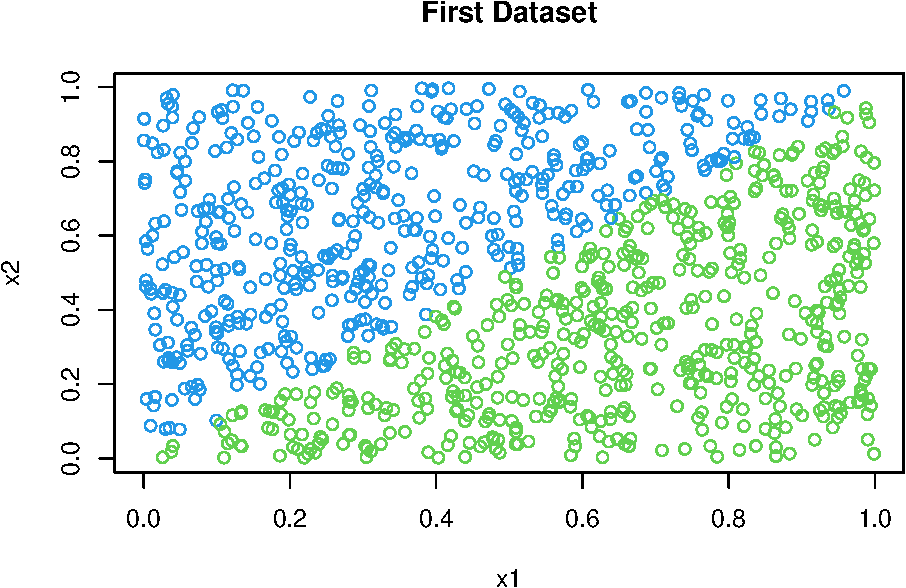
\includegraphics{Lab1Block2_files/figure-latex/1.7-1.pdf}
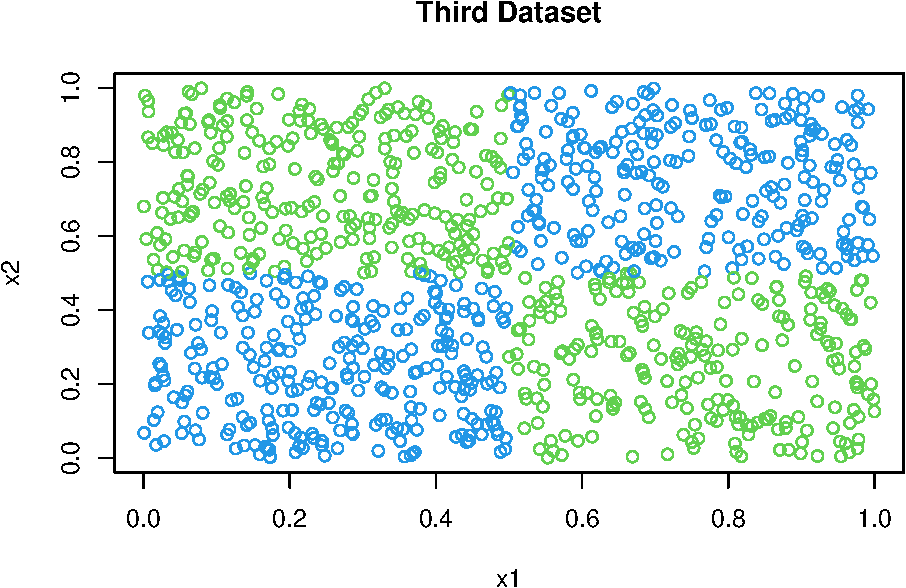
\includegraphics{Lab1Block2_files/figure-latex/1.7-2.pdf}

\hypertarget{assignment-2-mixture-models}{%
\subsection{Assignment 2: MIXTURE
MODELS}\label{assignment-2-mixture-models}}

\hypertarget{answer-1}{%
\subsubsection{Answer:}\label{answer-1}}

According to the question, bernoulli mixture model is:

\[
p(x) = \sum_{m=1}^{M}\pi_{m}  Bern(x|\mu_{m})
\]

where

\[
Bern(x|\mu_{m}) = \prod_{d=1}^{D} \mu_{m,d}^{x_{d}}(1-\mu_{m,d})^{1-x_{d}}
\]

And log-likelihood is:

\[
\sum_{i=1}^{n}log(p(x_{i}))
\]

Derivative of log-likelihood is:

\$\$

\sum\emph{\{i=1\}\^{}\{n\} \sum}\{m=1\}\^{}\{M\}\\
\$\$

According to the output, when we change M value to 2,3 and 4, the output
graph do not have significant change.

\begin{verbatim}
## Generate model when M= 2
\end{verbatim}

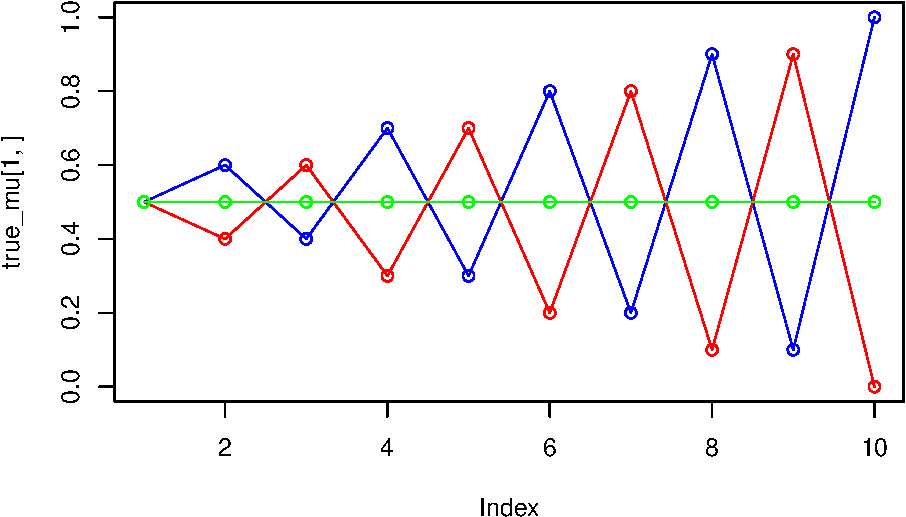
\includegraphics{Lab1Block2_files/figure-latex/unnamed-chunk-1-1.pdf}
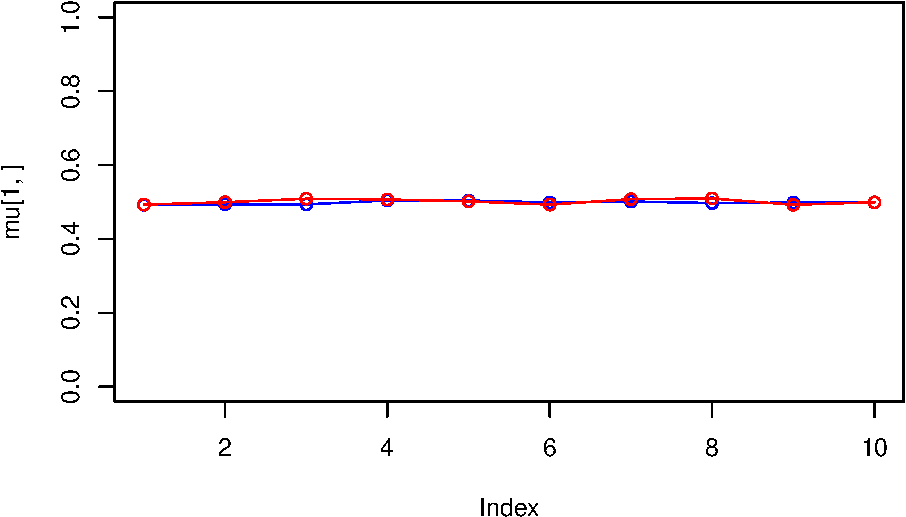
\includegraphics{Lab1Block2_files/figure-latex/unnamed-chunk-1-2.pdf}

\begin{verbatim}
## iteration:  1 log likelihood:  -6930.975
\end{verbatim}

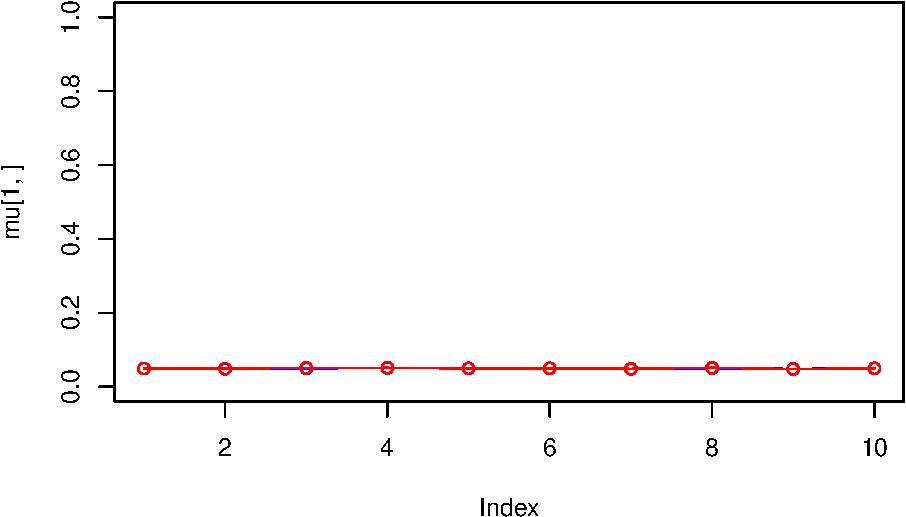
\includegraphics{Lab1Block2_files/figure-latex/unnamed-chunk-1-3.pdf}

\begin{verbatim}
## iteration:  2 log likelihood:  -15143.91
\end{verbatim}

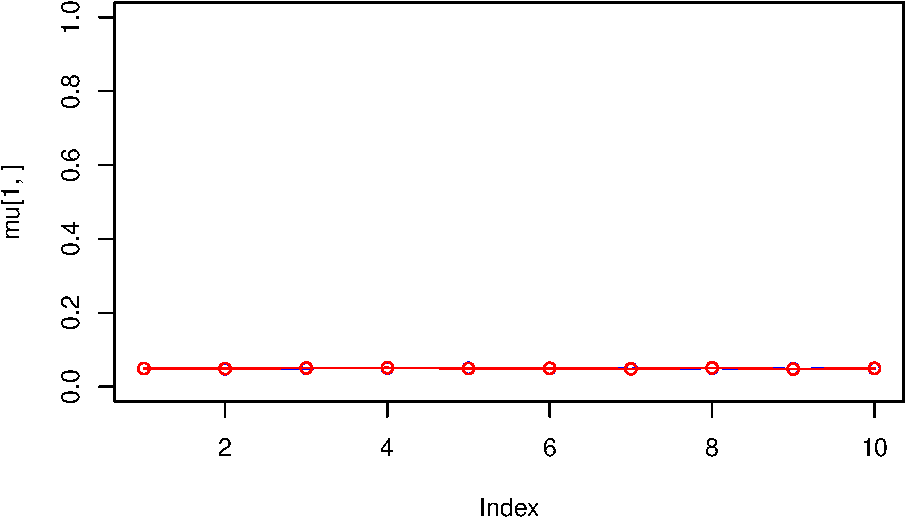
\includegraphics{Lab1Block2_files/figure-latex/unnamed-chunk-1-4.pdf}

\begin{verbatim}
## iteration:  3 log likelihood:  -15143.93
\end{verbatim}

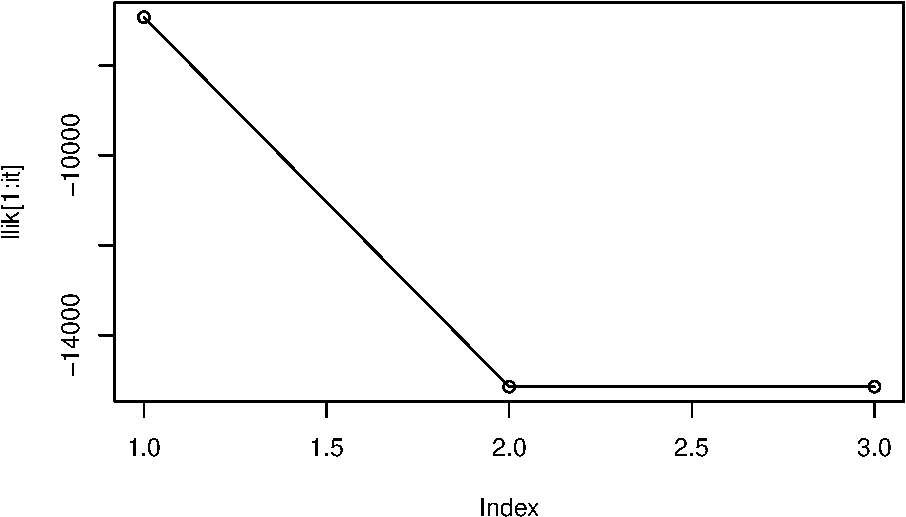
\includegraphics{Lab1Block2_files/figure-latex/unnamed-chunk-1-5.pdf}

\begin{verbatim}
## Generate model when M= 3
\end{verbatim}

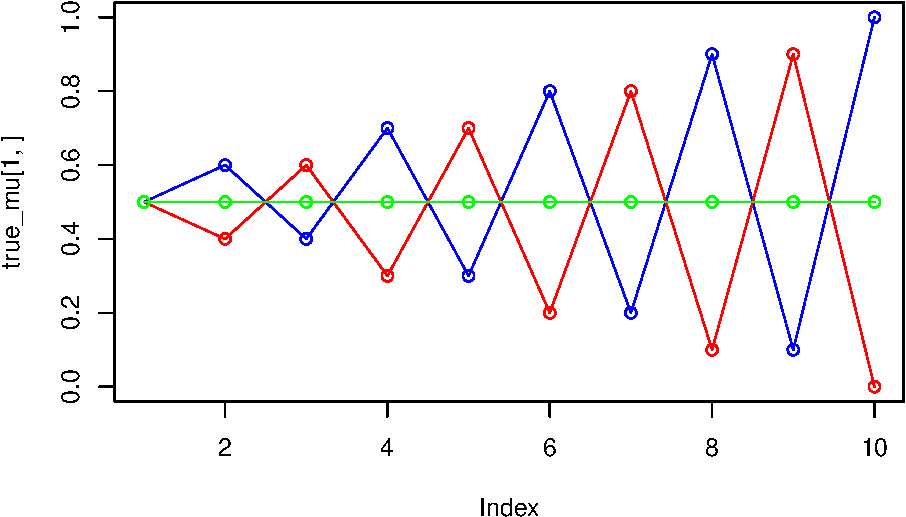
\includegraphics{Lab1Block2_files/figure-latex/unnamed-chunk-1-6.pdf}
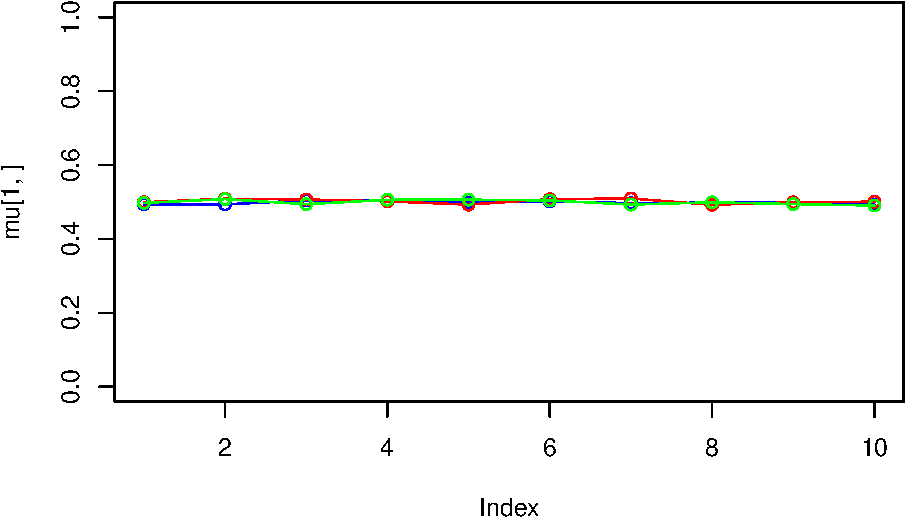
\includegraphics{Lab1Block2_files/figure-latex/unnamed-chunk-1-7.pdf}

\begin{verbatim}
## iteration:  1 log likelihood:  -6931.482
\end{verbatim}

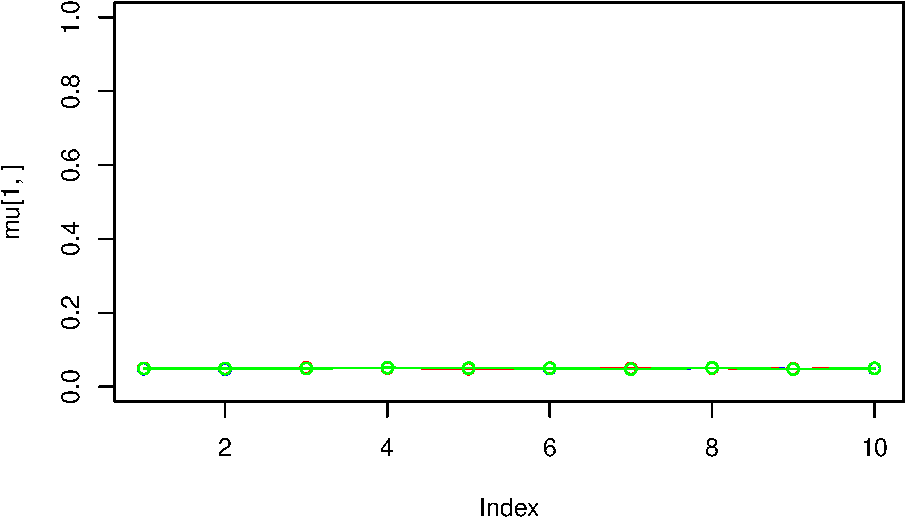
\includegraphics{Lab1Block2_files/figure-latex/unnamed-chunk-1-8.pdf}

\begin{verbatim}
## iteration:  2 log likelihood:  -15143.96
\end{verbatim}

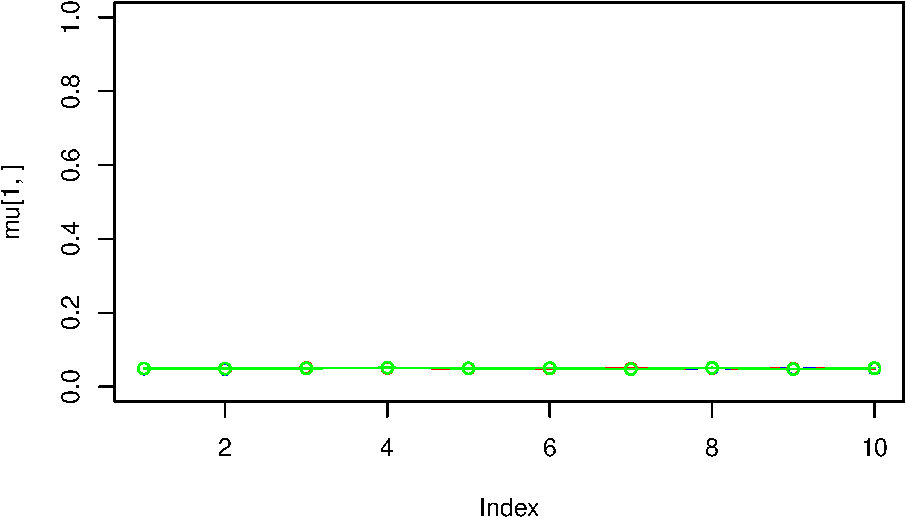
\includegraphics{Lab1Block2_files/figure-latex/unnamed-chunk-1-9.pdf}

\begin{verbatim}
## iteration:  3 log likelihood:  -15143.93
\end{verbatim}

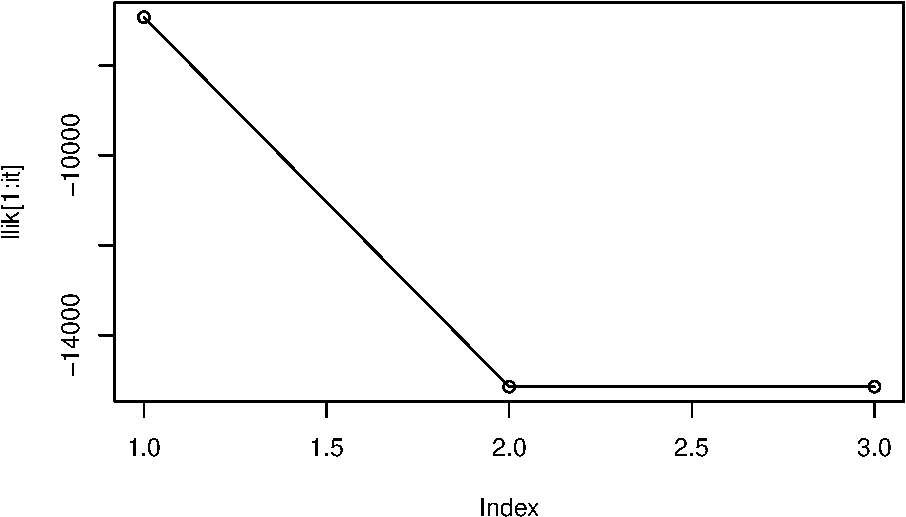
\includegraphics{Lab1Block2_files/figure-latex/unnamed-chunk-1-10.pdf}

\begin{verbatim}
## Generate model when M= 4
\end{verbatim}

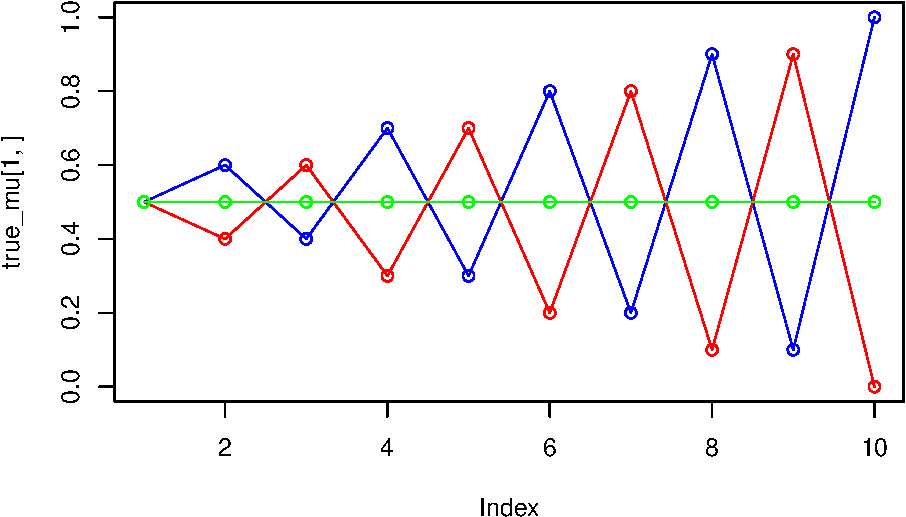
\includegraphics{Lab1Block2_files/figure-latex/unnamed-chunk-1-11.pdf}
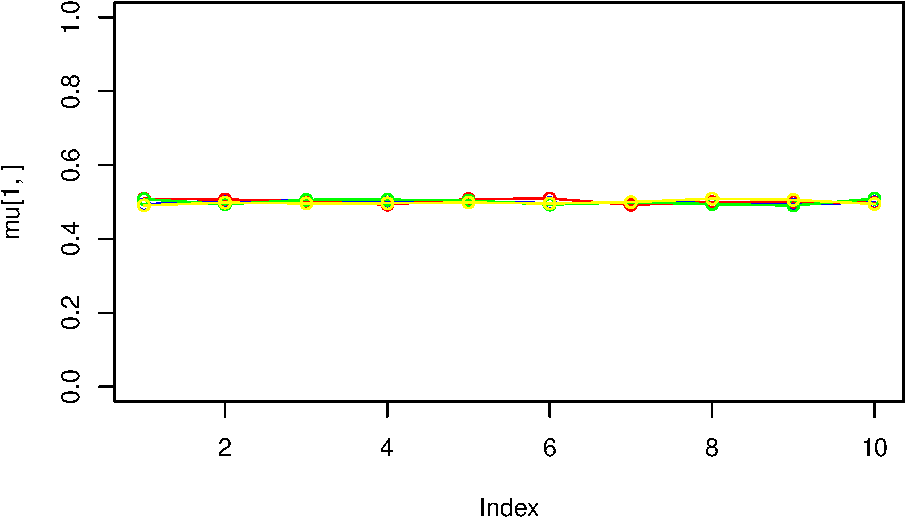
\includegraphics{Lab1Block2_files/figure-latex/unnamed-chunk-1-12.pdf}

\begin{verbatim}
## iteration:  1 log likelihood:  -6931.372
\end{verbatim}

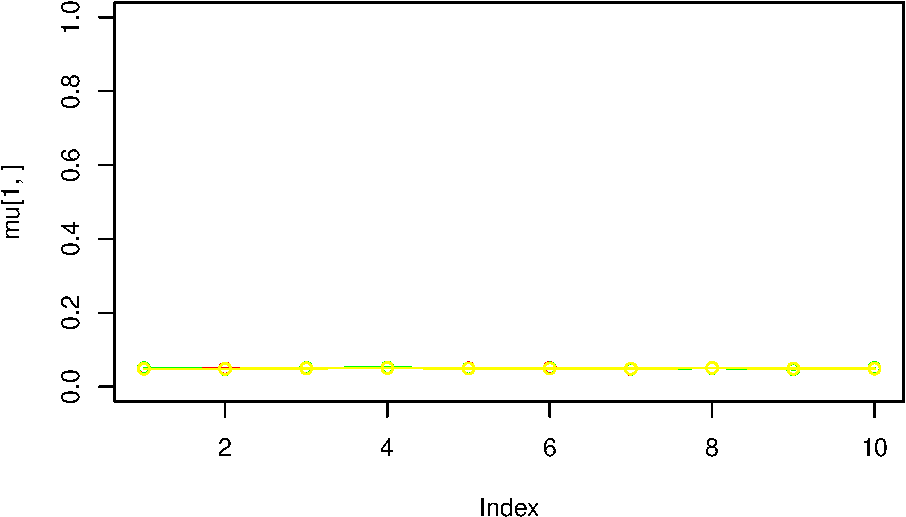
\includegraphics{Lab1Block2_files/figure-latex/unnamed-chunk-1-13.pdf}

\begin{verbatim}
## iteration:  2 log likelihood:  -15143.97
\end{verbatim}

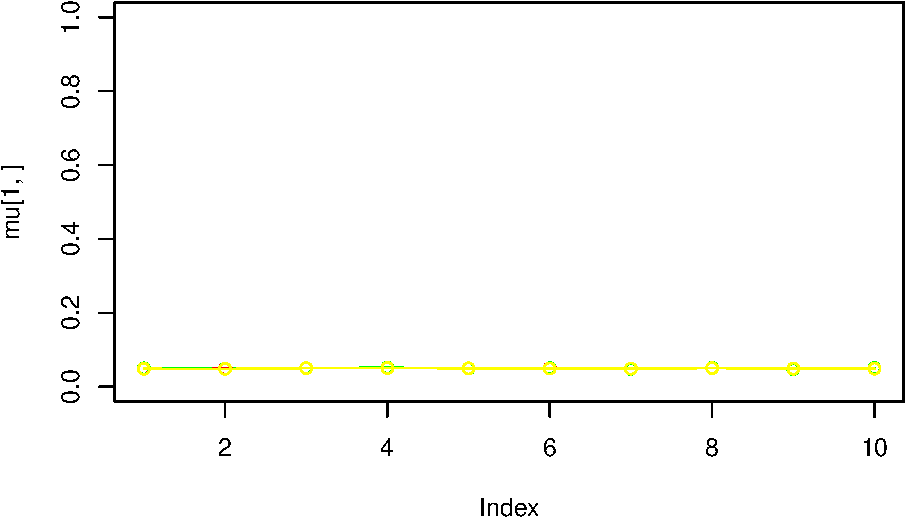
\includegraphics{Lab1Block2_files/figure-latex/unnamed-chunk-1-14.pdf}

\begin{verbatim}
## iteration:  3 log likelihood:  -15143.91
\end{verbatim}

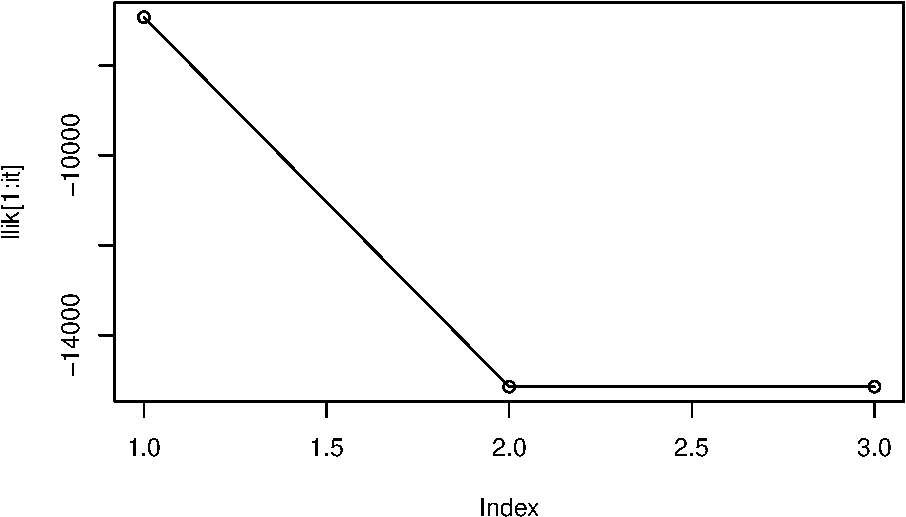
\includegraphics{Lab1Block2_files/figure-latex/unnamed-chunk-1-15.pdf}

\newpage

\hypertarget{appendix-all-code-for-this-report}{%
\section{Appendix: All code for this
report}\label{appendix-all-code-for-this-report}}

\begin{Shaded}
\begin{Highlighting}[]
\DocumentationTok{\#\#\#\#\#\#\#\#\#\#\#\#\#\#\#\#\#\#\#\#\#\#\#\#\#\#\#  Init code For Assignment 1 \#\#\#\#\#\#\#\#\#\#\#\#\#\#\#\#\#\#\#\#\#\#\#\#}
\FunctionTok{rm}\NormalTok{(}\AttributeTok{list =} \FunctionTok{ls}\NormalTok{())}
\NormalTok{knitr}\SpecialCharTok{::}\NormalTok{opts\_chunk}\SpecialCharTok{$}\FunctionTok{set}\NormalTok{(}\AttributeTok{echo =} \ConstantTok{TRUE}\NormalTok{)}
\FunctionTok{library}\NormalTok{(randomForest)}
\FunctionTok{set.seed}\NormalTok{(}\DecValTok{1234}\NormalTok{)}
\DocumentationTok{\#\#\#\#\#\#\#\#\#\#\#\#\#\#\#  Assignment 1 Ensemble methods \#\#\#\#\#\#\#\#\#\#\#\#\#\#\#\#\#\#\#\#\#\#\#\#\#\#\#\#\#\#\#\#\#}
\NormalTok{compare\_method1 }\OtherTok{\textless{}{-}} \ControlFlowTok{function}\NormalTok{(x1, x2) \{}
  \FunctionTok{return}\NormalTok{(x1 }\SpecialCharTok{\textless{}}\NormalTok{ x2)}
\NormalTok{\}}

\NormalTok{compare\_method2 }\OtherTok{\textless{}{-}} \ControlFlowTok{function}\NormalTok{(x1, x2) \{}
  \FunctionTok{return}\NormalTok{(x1 }\SpecialCharTok{\textless{}} \FloatTok{0.5}\NormalTok{)}
\NormalTok{\}}

\NormalTok{compare\_method3 }\OtherTok{\textless{}{-}} \ControlFlowTok{function}\NormalTok{(x1, x2) \{}
  \FunctionTok{return}\NormalTok{((x1 }\SpecialCharTok{\textgreater{}} \FloatTok{0.5} \SpecialCharTok{\&}\NormalTok{ x2 }\SpecialCharTok{\textgreater{}} \FloatTok{0.5}\NormalTok{) }\SpecialCharTok{|}\NormalTok{ (x1 }\SpecialCharTok{\textless{}} \FloatTok{0.5} \SpecialCharTok{\&}\NormalTok{ x2 }\SpecialCharTok{\textless{}} \FloatTok{0.5}\NormalTok{))}
\NormalTok{\}}

\NormalTok{ensemble\_method }\OtherTok{\textless{}{-}} \ControlFlowTok{function}\NormalTok{(record\_number, tree\_number, node\_size, compare\_method) \{}
  \CommentTok{\# init data set (copy from pdf file)}
  
\NormalTok{  x1 }\OtherTok{\textless{}{-}} \FunctionTok{runif}\NormalTok{(}\DecValTok{100}\NormalTok{)  }
\NormalTok{  x2 }\OtherTok{\textless{}{-}} \FunctionTok{runif}\NormalTok{(}\DecValTok{100}\NormalTok{)}

\NormalTok{  trdata }\OtherTok{\textless{}{-}} \FunctionTok{cbind}\NormalTok{(x1, x2)}
\NormalTok{  y }\OtherTok{\textless{}{-}} \FunctionTok{as.numeric}\NormalTok{(}\FunctionTok{compare\_method}\NormalTok{(x1, x2))}
\NormalTok{  trlabels }\OtherTok{\textless{}{-}} \FunctionTok{as.factor}\NormalTok{(y)}
\NormalTok{  trdata }\OtherTok{\textless{}{-}} \FunctionTok{cbind}\NormalTok{(trdata, trlabels)}
  
  \CommentTok{\# training the model using random forest}
\NormalTok{  rf\_model }\OtherTok{\textless{}{-}} \FunctionTok{randomForest}\NormalTok{( }\FunctionTok{as.factor}\NormalTok{(trlabels) }\SpecialCharTok{\textasciitilde{}}\NormalTok{ ., }
                            \AttributeTok{data =}\NormalTok{ trdata, }
                            \AttributeTok{ntree =}\NormalTok{ tree\_number,}
                            \AttributeTok{nodesize =}\NormalTok{ node\_size, }
                            \AttributeTok{keep.forest =} \ConstantTok{TRUE}\NormalTok{)}


\NormalTok{  x1 }\OtherTok{\textless{}{-}} \FunctionTok{runif}\NormalTok{(record\_number)}
\NormalTok{  x2 }\OtherTok{\textless{}{-}} \FunctionTok{runif}\NormalTok{(record\_number)}
\NormalTok{  tedata }\OtherTok{\textless{}{-}} \FunctionTok{cbind}\NormalTok{(x1, x2)}
\NormalTok{  y }\OtherTok{\textless{}{-}} \FunctionTok{as.numeric}\NormalTok{(}\FunctionTok{compare\_method}\NormalTok{(x1, x2))}
\NormalTok{  telabels }\OtherTok{\textless{}{-}} \FunctionTok{as.factor}\NormalTok{(y)}

\NormalTok{  rf\_pred }\OtherTok{\textless{}{-}} \FunctionTok{predict}\NormalTok{(rf\_model, }\AttributeTok{newdata =}\NormalTok{ tedata, }\AttributeTok{type =} \StringTok{"class"}\NormalTok{)}
  
  \CommentTok{\# calculate the misclassification rate  }
\NormalTok{  misclassification\_rate }\OtherTok{\textless{}{-}} \DecValTok{1}\SpecialCharTok{{-}} \FunctionTok{sum}\NormalTok{(}\FunctionTok{diag}\NormalTok{(}\FunctionTok{table}\NormalTok{(rf\_pred ,telabels)))}\SpecialCharTok{/}\FunctionTok{length}\NormalTok{(rf\_pred)}

  \FunctionTok{return}\NormalTok{ (misclassification\_rate)}
\NormalTok{\}}


\DocumentationTok{\#\#\#\#\#\#\#\#\#\#\#\#\#\#\#\#\#\#\#\#\#\#\#\#\#\#\#\#\#\#\#\#\#\#\#\#\#\#\#\#\#\#\#\#\#\#\#\#\#\#\#\#\#\#\#\#\#\#\#\#\#\#\#\#\#\#\#\#\#\#\#\#\#\#\#\#\#\#\#\#}
\CommentTok{\# call the function}
\NormalTok{record\_numbers }\OtherTok{\textless{}{-}} \FunctionTok{c}\NormalTok{(}\DecValTok{100}\NormalTok{, }\DecValTok{1000}\NormalTok{)}
\NormalTok{tree\_numbers }\OtherTok{\textless{}{-}} \FunctionTok{c}\NormalTok{(}\DecValTok{1}\NormalTok{, }\DecValTok{10}\NormalTok{, }\DecValTok{100}\NormalTok{)}

\NormalTok{node\_size }\OtherTok{\textless{}{-}} \DecValTok{25}
\CommentTok{\# data record number = 100}
\NormalTok{result1 }\OtherTok{\textless{}{-}} \FunctionTok{ensemble\_method}\NormalTok{(record\_numbers[}\DecValTok{1}\NormalTok{], tree\_numbers[}\DecValTok{1}\NormalTok{], node\_size, }
\NormalTok{                          compare\_method1)}
\NormalTok{result2 }\OtherTok{\textless{}{-}} \FunctionTok{ensemble\_method}\NormalTok{(record\_numbers[}\DecValTok{1}\NormalTok{], tree\_numbers[}\DecValTok{2}\NormalTok{], node\_size, }
\NormalTok{                          compare\_method1)}
\NormalTok{result3 }\OtherTok{\textless{}{-}} \FunctionTok{ensemble\_method}\NormalTok{(record\_numbers[}\DecValTok{1}\NormalTok{], tree\_numbers[}\DecValTok{3}\NormalTok{], node\_size, }
\NormalTok{                          compare\_method1)}

\NormalTok{misclassification\_df }\OtherTok{\textless{}{-}} \FunctionTok{data.frame}\NormalTok{(}\FunctionTok{matrix}\NormalTok{(}\AttributeTok{ncol =} \DecValTok{2}\NormalTok{, }\AttributeTok{nrow=}\DecValTok{0}\NormalTok{))}
\FunctionTok{colnames}\NormalTok{(misclassification\_df) }\OtherTok{\textless{}{-}} \FunctionTok{c}\NormalTok{(}\StringTok{"tree\_number"}\NormalTok{, }\StringTok{"misclassification\_rate"}\NormalTok{)}

\NormalTok{misclassification\_df }\OtherTok{\textless{}{-}} \FunctionTok{rbind}\NormalTok{(misclassification\_df, }\FunctionTok{data.frame}\NormalTok{(}\StringTok{"tree\_number"} \OtherTok{=}\NormalTok{ tree\_numbers[}\DecValTok{1}\NormalTok{], }\StringTok{"misclassification\_rate"} \OtherTok{=}\NormalTok{ result1))  }
\NormalTok{misclassification\_df }\OtherTok{\textless{}{-}} \FunctionTok{rbind}\NormalTok{(misclassification\_df, }\FunctionTok{data.frame}\NormalTok{(}\StringTok{"tree\_number"} \OtherTok{=}\NormalTok{ tree\_numbers[}\DecValTok{2}\NormalTok{], }\StringTok{"misclassification\_rate"} \OtherTok{=}\NormalTok{ result2))  }
\NormalTok{misclassification\_df }\OtherTok{\textless{}{-}} \FunctionTok{rbind}\NormalTok{(misclassification\_df, }\FunctionTok{data.frame}\NormalTok{(}\StringTok{"tree\_number"} \OtherTok{=}\NormalTok{ tree\_numbers[}\DecValTok{3}\NormalTok{], }\StringTok{"misclassification\_rate"} \OtherTok{=}\NormalTok{ result3))  }

\NormalTok{misclassification\_df}
\DocumentationTok{\#\#\#\#\#\#\#\#\#\#\#\#\#\#\#\#\#\#\#\#\#\#\#\#\#\#\#\#\#\#\#\#\#\#\#\#\#\#\#\#\#\#\#\#\#\#\#\#\#\#\#\#\#\#\#\#\#\#\#\#\#\#\#\#\#\#\#\#\#\#\#\#\#\#\#\#\#\#\#\#}
\CommentTok{\# When we set node\_size = 25 and record\_numbers = 100 and 1000 and check x1 \textless{} x2 ,and tree\_num = 1,10,100}
\CommentTok{\# and run it 1000 times}

\NormalTok{misclassification\_rates\_1}\FloatTok{.1} \OtherTok{\textless{}{-}} \FunctionTok{rep}\NormalTok{(}\DecValTok{0}\NormalTok{, }\DecValTok{1000}\NormalTok{)}
\NormalTok{misclassification\_rates\_10}\FloatTok{.1} \OtherTok{\textless{}{-}} \FunctionTok{rep}\NormalTok{(}\DecValTok{0}\NormalTok{, }\DecValTok{1000}\NormalTok{)}
\NormalTok{misclassification\_rates\_100}\FloatTok{.1} \OtherTok{\textless{}{-}} \FunctionTok{rep}\NormalTok{(}\DecValTok{0}\NormalTok{, }\DecValTok{1000}\NormalTok{)}

\NormalTok{misclassification\_rates\_1}\FloatTok{.2} \OtherTok{\textless{}{-}} \FunctionTok{rep}\NormalTok{(}\DecValTok{0}\NormalTok{, }\DecValTok{1000}\NormalTok{)}
\NormalTok{misclassification\_rates\_10}\FloatTok{.2} \OtherTok{\textless{}{-}} \FunctionTok{rep}\NormalTok{(}\DecValTok{0}\NormalTok{, }\DecValTok{1000}\NormalTok{)}
\NormalTok{misclassification\_rates\_100}\FloatTok{.2} \OtherTok{\textless{}{-}} \FunctionTok{rep}\NormalTok{(}\DecValTok{0}\NormalTok{, }\DecValTok{1000}\NormalTok{)}

\NormalTok{node\_size }\OtherTok{=} \DecValTok{25}
\ControlFlowTok{for}\NormalTok{ (i }\ControlFlowTok{in} \DecValTok{1}\SpecialCharTok{:}\DecValTok{1000}\NormalTok{) \{}

  \CommentTok{\# data record number = 100}
\NormalTok{  misclassification\_rates\_1}\FloatTok{.1}\NormalTok{[i] }\OtherTok{\textless{}{-}} \FunctionTok{ensemble\_method}\NormalTok{(record\_numbers[}\DecValTok{1}\NormalTok{], }
\NormalTok{                                                 tree\_numbers[}\DecValTok{1}\NormalTok{], node\_size, }
\NormalTok{                                                 compare\_method1)}
\NormalTok{  misclassification\_rates\_10}\FloatTok{.1}\NormalTok{[i] }\OtherTok{\textless{}{-}} \FunctionTok{ensemble\_method}\NormalTok{(record\_numbers[}\DecValTok{1}\NormalTok{], }
\NormalTok{                                                  tree\_numbers[}\DecValTok{2}\NormalTok{], node\_size, }
\NormalTok{                                                  compare\_method1)}
\NormalTok{  misclassification\_rates\_100}\FloatTok{.1}\NormalTok{[i] }\OtherTok{\textless{}{-}} \FunctionTok{ensemble\_method}\NormalTok{(record\_numbers[}\DecValTok{1}\NormalTok{], }
\NormalTok{                                                   tree\_numbers[}\DecValTok{3}\NormalTok{], node\_size, }
\NormalTok{                                                compare\_method1)}
  \CommentTok{\# data record number = 1000}
\NormalTok{  misclassification\_rates\_1}\FloatTok{.2}\NormalTok{[i] }\OtherTok{\textless{}{-}} \FunctionTok{ensemble\_method}\NormalTok{(record\_numbers[}\DecValTok{2}\NormalTok{], }
\NormalTok{                                                 tree\_numbers[}\DecValTok{1}\NormalTok{], node\_size, }
\NormalTok{                                                 compare\_method1)}
\NormalTok{  misclassification\_rates\_10}\FloatTok{.2}\NormalTok{[i] }\OtherTok{\textless{}{-}} \FunctionTok{ensemble\_method}\NormalTok{(record\_numbers[}\DecValTok{2}\NormalTok{], }
\NormalTok{                                                  tree\_numbers[}\DecValTok{2}\NormalTok{], node\_size, }
\NormalTok{                                                  compare\_method1)}
\NormalTok{  misclassification\_rates\_100}\FloatTok{.2}\NormalTok{[i] }\OtherTok{\textless{}{-}} \FunctionTok{ensemble\_method}\NormalTok{(record\_numbers[}\DecValTok{2}\NormalTok{], }
\NormalTok{                                                   tree\_numbers[}\DecValTok{3}\NormalTok{], node\_size, }
\NormalTok{                                                compare\_method1)}
\NormalTok{\}}

\NormalTok{misclassification\_mean\_var\_df }\OtherTok{\textless{}{-}} \FunctionTok{data.frame}\NormalTok{(}\FunctionTok{matrix}\NormalTok{(}\AttributeTok{ncol =} \DecValTok{4}\NormalTok{, }\AttributeTok{nrow=}\DecValTok{0}\NormalTok{))}
\FunctionTok{colnames}\NormalTok{(misclassification\_mean\_var\_df) }\OtherTok{\textless{}{-}} \FunctionTok{c}\NormalTok{(}\StringTok{"tree\_number"}\NormalTok{, }\StringTok{"record\_number"}\NormalTok{, }\StringTok{"misclassification\_mean"}\NormalTok{, }\StringTok{"misclassification\_var"}\NormalTok{) }

\NormalTok{misclassification\_mean\_var\_df }\OtherTok{\textless{}{-}} \FunctionTok{rbind}\NormalTok{(misclassification\_mean\_var\_df, }
                                      \FunctionTok{data.frame}\NormalTok{(}\StringTok{"tree\_number"} \OtherTok{=} \DecValTok{1}\NormalTok{, }
                                                 \StringTok{"record\_number"} \OtherTok{=} \DecValTok{100}\NormalTok{,}
                                                 \StringTok{"misclassification\_mean"} \OtherTok{=} \FunctionTok{mean}\NormalTok{(misclassification\_rates\_1}\FloatTok{.1}\NormalTok{),}
                                                 \StringTok{"misclassification\_var"} \OtherTok{=} \FunctionTok{var}\NormalTok{(misclassification\_rates\_1}\FloatTok{.1}\NormalTok{)}
\NormalTok{                                                 ))}

\NormalTok{misclassification\_mean\_var\_df }\OtherTok{\textless{}{-}} \FunctionTok{rbind}\NormalTok{(misclassification\_mean\_var\_df, }
                                      \FunctionTok{data.frame}\NormalTok{(}\StringTok{"tree\_number"} \OtherTok{=} \DecValTok{10}\NormalTok{, }
                                                 \StringTok{"record\_number"} \OtherTok{=} \DecValTok{100}\NormalTok{,}
                                                 \StringTok{"misclassification\_mean"} \OtherTok{=} \FunctionTok{mean}\NormalTok{(misclassification\_rates\_10}\FloatTok{.1}\NormalTok{),}
                                                 \StringTok{"misclassification\_var"} \OtherTok{=} \FunctionTok{var}\NormalTok{(misclassification\_rates\_10}\FloatTok{.1}\NormalTok{)}
\NormalTok{                                                 ))}

\NormalTok{misclassification\_mean\_var\_df }\OtherTok{\textless{}{-}} \FunctionTok{rbind}\NormalTok{(misclassification\_mean\_var\_df, }
                                      \FunctionTok{data.frame}\NormalTok{(}\StringTok{"tree\_number"} \OtherTok{=} \DecValTok{100}\NormalTok{, }
                                                 \StringTok{"record\_number"} \OtherTok{=} \DecValTok{100}\NormalTok{,}
                                                 \StringTok{"misclassification\_mean"} \OtherTok{=} \FunctionTok{mean}\NormalTok{(misclassification\_rates\_100}\FloatTok{.1}\NormalTok{),}
                                                 \StringTok{"misclassification\_var"} \OtherTok{=} \FunctionTok{var}\NormalTok{(misclassification\_rates\_100}\FloatTok{.1}\NormalTok{)}
\NormalTok{                                                 ))}

\NormalTok{misclassification\_mean\_var\_df }\OtherTok{\textless{}{-}} \FunctionTok{rbind}\NormalTok{(misclassification\_mean\_var\_df, }
                                      \FunctionTok{data.frame}\NormalTok{(}\StringTok{"tree\_number"} \OtherTok{=} \DecValTok{1}\NormalTok{, }
                                                 \StringTok{"record\_number"} \OtherTok{=} \DecValTok{1000}\NormalTok{,}
                                                 \StringTok{"misclassification\_mean"} \OtherTok{=} \FunctionTok{mean}\NormalTok{(misclassification\_rates\_1}\FloatTok{.2}\NormalTok{),}
                                                 \StringTok{"misclassification\_var"} \OtherTok{=} \FunctionTok{var}\NormalTok{(misclassification\_rates\_1}\FloatTok{.2}\NormalTok{)}
\NormalTok{                                                 ))}

\NormalTok{misclassification\_mean\_var\_df }\OtherTok{\textless{}{-}} \FunctionTok{rbind}\NormalTok{(misclassification\_mean\_var\_df, }
                                      \FunctionTok{data.frame}\NormalTok{(}\StringTok{"tree\_number"} \OtherTok{=} \DecValTok{10}\NormalTok{, }
                                                 \StringTok{"record\_number"} \OtherTok{=} \DecValTok{1000}\NormalTok{,}
                                                 \StringTok{"misclassification\_mean"} \OtherTok{=} \FunctionTok{mean}\NormalTok{(misclassification\_rates\_10}\FloatTok{.2}\NormalTok{),}
                                                 \StringTok{"misclassification\_var"} \OtherTok{=} \FunctionTok{var}\NormalTok{(misclassification\_rates\_10}\FloatTok{.2}\NormalTok{)}
\NormalTok{                                                 ))}

\NormalTok{misclassification\_mean\_var\_df }\OtherTok{\textless{}{-}} \FunctionTok{rbind}\NormalTok{(misclassification\_mean\_var\_df, }
                                      \FunctionTok{data.frame}\NormalTok{(}\StringTok{"tree\_number"} \OtherTok{=} \DecValTok{100}\NormalTok{, }
                                                 \StringTok{"record\_number"} \OtherTok{=} \DecValTok{1000}\NormalTok{,}
                                                 \StringTok{"misclassification\_mean"} \OtherTok{=} \FunctionTok{mean}\NormalTok{(misclassification\_rates\_100}\FloatTok{.2}\NormalTok{),}
                                                 \StringTok{"misclassification\_var"} \OtherTok{=} \FunctionTok{var}\NormalTok{(misclassification\_rates\_100}\FloatTok{.2}\NormalTok{)}
\NormalTok{                                                 ))}

\NormalTok{misclassification\_mean\_var\_df}
\DocumentationTok{\#\#\#\#\#\#\#\#\#\#\#\#\#\#\#\#\#\#\#\#\#\#\#\#\#\#\#\#\#\#\#\#\#\#\#\#\#\#\#\#\#\#\#\#\#\#\#\#\#\#\#\#\#\#\#\#\#\#\#\#\#\#\#\#\#\#\#\#\#\#\#\#\#\#\#\#\#\#\#\#}
\CommentTok{\# When we set node\_size = 25 and record\_numbers = 100 and 1000 and check x1 \textless{} 0.5 ,and tree\_num = 1,10,100}
\CommentTok{\# and run it 1000 times}

\NormalTok{misclassification\_rates\_1}\FloatTok{.1} \OtherTok{\textless{}{-}} \FunctionTok{rep}\NormalTok{(}\DecValTok{0}\NormalTok{, }\DecValTok{1000}\NormalTok{)}
\NormalTok{misclassification\_rates\_10}\FloatTok{.1} \OtherTok{\textless{}{-}} \FunctionTok{rep}\NormalTok{(}\DecValTok{0}\NormalTok{, }\DecValTok{1000}\NormalTok{)}
\NormalTok{misclassification\_rates\_100}\FloatTok{.1} \OtherTok{\textless{}{-}} \FunctionTok{rep}\NormalTok{(}\DecValTok{0}\NormalTok{, }\DecValTok{1000}\NormalTok{)}

\NormalTok{misclassification\_rates\_1}\FloatTok{.2} \OtherTok{\textless{}{-}} \FunctionTok{rep}\NormalTok{(}\DecValTok{0}\NormalTok{, }\DecValTok{1000}\NormalTok{)}
\NormalTok{misclassification\_rates\_10}\FloatTok{.2} \OtherTok{\textless{}{-}} \FunctionTok{rep}\NormalTok{(}\DecValTok{0}\NormalTok{, }\DecValTok{1000}\NormalTok{)}
\NormalTok{misclassification\_rates\_100}\FloatTok{.2} \OtherTok{\textless{}{-}} \FunctionTok{rep}\NormalTok{(}\DecValTok{0}\NormalTok{, }\DecValTok{1000}\NormalTok{)}

\NormalTok{node\_size }\OtherTok{=} \DecValTok{25}
\ControlFlowTok{for}\NormalTok{ (i }\ControlFlowTok{in} \DecValTok{1}\SpecialCharTok{:}\DecValTok{1000}\NormalTok{) \{}

  \CommentTok{\# data record number = 100}
\NormalTok{  misclassification\_rates\_1}\FloatTok{.1}\NormalTok{[i] }\OtherTok{\textless{}{-}} \FunctionTok{ensemble\_method}\NormalTok{(record\_numbers[}\DecValTok{1}\NormalTok{], }
\NormalTok{                                                 tree\_numbers[}\DecValTok{1}\NormalTok{], node\_size, }
\NormalTok{                                                 compare\_method2)}
\NormalTok{  misclassification\_rates\_10}\FloatTok{.1}\NormalTok{[i] }\OtherTok{\textless{}{-}} \FunctionTok{ensemble\_method}\NormalTok{(record\_numbers[}\DecValTok{1}\NormalTok{], }
\NormalTok{                                                  tree\_numbers[}\DecValTok{2}\NormalTok{], node\_size, }
\NormalTok{                                                  compare\_method2)}
\NormalTok{  misclassification\_rates\_100}\FloatTok{.1}\NormalTok{[i] }\OtherTok{\textless{}{-}} \FunctionTok{ensemble\_method}\NormalTok{(record\_numbers[}\DecValTok{1}\NormalTok{], }
\NormalTok{                                                   tree\_numbers[}\DecValTok{3}\NormalTok{], node\_size, }
\NormalTok{                                                compare\_method2)}
  \CommentTok{\# data record number = 1000}
\NormalTok{  misclassification\_rates\_1}\FloatTok{.2}\NormalTok{[i] }\OtherTok{\textless{}{-}} \FunctionTok{ensemble\_method}\NormalTok{(record\_numbers[}\DecValTok{2}\NormalTok{], }
\NormalTok{                                                 tree\_numbers[}\DecValTok{1}\NormalTok{], node\_size, }
\NormalTok{                                                 compare\_method2)}
\NormalTok{  misclassification\_rates\_10}\FloatTok{.2}\NormalTok{[i] }\OtherTok{\textless{}{-}} \FunctionTok{ensemble\_method}\NormalTok{(record\_numbers[}\DecValTok{2}\NormalTok{], }
\NormalTok{                                                  tree\_numbers[}\DecValTok{2}\NormalTok{], node\_size, }
\NormalTok{                                                  compare\_method2)}
\NormalTok{  misclassification\_rates\_100}\FloatTok{.2}\NormalTok{[i] }\OtherTok{\textless{}{-}} \FunctionTok{ensemble\_method}\NormalTok{(record\_numbers[}\DecValTok{2}\NormalTok{], }
\NormalTok{                                                   tree\_numbers[}\DecValTok{3}\NormalTok{], node\_size, }
\NormalTok{                                                compare\_method2)}
\NormalTok{\}}

\NormalTok{misclassification\_mean\_var\_df }\OtherTok{\textless{}{-}} \FunctionTok{data.frame}\NormalTok{(}\FunctionTok{matrix}\NormalTok{(}\AttributeTok{ncol =} \DecValTok{4}\NormalTok{, }\AttributeTok{nrow=}\DecValTok{0}\NormalTok{))}
\FunctionTok{colnames}\NormalTok{(misclassification\_mean\_var\_df) }\OtherTok{\textless{}{-}} \FunctionTok{c}\NormalTok{(}\StringTok{"tree\_number"}\NormalTok{, }\StringTok{"record\_number"}\NormalTok{, }\StringTok{"misclassification\_mean"}\NormalTok{, }\StringTok{"misclassification\_var"}\NormalTok{) }

\NormalTok{misclassification\_mean\_var\_df }\OtherTok{\textless{}{-}} \FunctionTok{rbind}\NormalTok{(misclassification\_mean\_var\_df, }
                                      \FunctionTok{data.frame}\NormalTok{(}\StringTok{"tree\_number"} \OtherTok{=} \DecValTok{1}\NormalTok{, }
                                                 \StringTok{"record\_number"} \OtherTok{=} \DecValTok{100}\NormalTok{,}
                                                 \StringTok{"misclassification\_mean"} \OtherTok{=} \FunctionTok{mean}\NormalTok{(misclassification\_rates\_1}\FloatTok{.1}\NormalTok{),}
                                                 \StringTok{"misclassification\_var"} \OtherTok{=} \FunctionTok{var}\NormalTok{(misclassification\_rates\_1}\FloatTok{.1}\NormalTok{)}
\NormalTok{                                                 ))}

\NormalTok{misclassification\_mean\_var\_df }\OtherTok{\textless{}{-}} \FunctionTok{rbind}\NormalTok{(misclassification\_mean\_var\_df, }
                                      \FunctionTok{data.frame}\NormalTok{(}\StringTok{"tree\_number"} \OtherTok{=} \DecValTok{10}\NormalTok{, }
                                                 \StringTok{"record\_number"} \OtherTok{=} \DecValTok{100}\NormalTok{,}
                                                 \StringTok{"misclassification\_mean"} \OtherTok{=} \FunctionTok{mean}\NormalTok{(misclassification\_rates\_10}\FloatTok{.1}\NormalTok{),}
                                                 \StringTok{"misclassification\_var"} \OtherTok{=} \FunctionTok{var}\NormalTok{(misclassification\_rates\_10}\FloatTok{.1}\NormalTok{)}
\NormalTok{                                                 ))}

\NormalTok{misclassification\_mean\_var\_df }\OtherTok{\textless{}{-}} \FunctionTok{rbind}\NormalTok{(misclassification\_mean\_var\_df, }
                                      \FunctionTok{data.frame}\NormalTok{(}\StringTok{"tree\_number"} \OtherTok{=} \DecValTok{100}\NormalTok{, }
                                                 \StringTok{"record\_number"} \OtherTok{=} \DecValTok{100}\NormalTok{,}
                                                 \StringTok{"misclassification\_mean"} \OtherTok{=} \FunctionTok{mean}\NormalTok{(misclassification\_rates\_100}\FloatTok{.1}\NormalTok{),}
                                                 \StringTok{"misclassification\_var"} \OtherTok{=} \FunctionTok{var}\NormalTok{(misclassification\_rates\_100}\FloatTok{.1}\NormalTok{)}
\NormalTok{                                                 ))}

\NormalTok{misclassification\_mean\_var\_df }\OtherTok{\textless{}{-}} \FunctionTok{rbind}\NormalTok{(misclassification\_mean\_var\_df, }
                                      \FunctionTok{data.frame}\NormalTok{(}\StringTok{"tree\_number"} \OtherTok{=} \DecValTok{1}\NormalTok{, }
                                                 \StringTok{"record\_number"} \OtherTok{=} \DecValTok{1000}\NormalTok{,}
                                                 \StringTok{"misclassification\_mean"} \OtherTok{=} \FunctionTok{mean}\NormalTok{(misclassification\_rates\_1}\FloatTok{.2}\NormalTok{),}
                                                 \StringTok{"misclassification\_var"} \OtherTok{=} \FunctionTok{var}\NormalTok{(misclassification\_rates\_1}\FloatTok{.2}\NormalTok{)}
\NormalTok{                                                 ))}

\NormalTok{misclassification\_mean\_var\_df }\OtherTok{\textless{}{-}} \FunctionTok{rbind}\NormalTok{(misclassification\_mean\_var\_df, }
                                      \FunctionTok{data.frame}\NormalTok{(}\StringTok{"tree\_number"} \OtherTok{=} \DecValTok{10}\NormalTok{, }
                                                 \StringTok{"record\_number"} \OtherTok{=} \DecValTok{1000}\NormalTok{,}
                                                 \StringTok{"misclassification\_mean"} \OtherTok{=} \FunctionTok{mean}\NormalTok{(misclassification\_rates\_10}\FloatTok{.2}\NormalTok{),}
                                                 \StringTok{"misclassification\_var"} \OtherTok{=} \FunctionTok{var}\NormalTok{(misclassification\_rates\_10}\FloatTok{.2}\NormalTok{)}
\NormalTok{                                                 ))}

\NormalTok{misclassification\_mean\_var\_df }\OtherTok{\textless{}{-}} \FunctionTok{rbind}\NormalTok{(misclassification\_mean\_var\_df, }
                                      \FunctionTok{data.frame}\NormalTok{(}\StringTok{"tree\_number"} \OtherTok{=} \DecValTok{100}\NormalTok{, }
                                                 \StringTok{"record\_number"} \OtherTok{=} \DecValTok{1000}\NormalTok{,}
                                                 \StringTok{"misclassification\_mean"} \OtherTok{=} \FunctionTok{mean}\NormalTok{(misclassification\_rates\_100}\FloatTok{.2}\NormalTok{),}
                                                 \StringTok{"misclassification\_var"} \OtherTok{=} \FunctionTok{var}\NormalTok{(misclassification\_rates\_100}\FloatTok{.2}\NormalTok{)}
\NormalTok{                                                 ))}

\NormalTok{misclassification\_mean\_var\_df}
\DocumentationTok{\#\#\#\#\#\#\#\#\#\#\#\#\#\#\#\#\#\#\#\#\#\#\#\#\#\#\#\#\#\#\#\#\#\#\#\#\#\#\#\#\#\#\#\#\#\#\#\#\#\#\#\#\#\#\#\#\#\#\#\#\#\#\#\#\#\#\#\#\#\#\#\#\#\#\#\#\#\#\#\#}
\CommentTok{\# When we set node\_size = 12 and record\_numbers = 100 and check }
\CommentTok{\#((x1 \textgreater{} 0.5 \& x2 \textgreater{} 0.5) | (x1 \textless{} 0.5 \& x2 \textless{} 0.5)) , and run  it 1000 times}

\NormalTok{misclassification\_rates\_1}\FloatTok{.1} \OtherTok{\textless{}{-}} \FunctionTok{rep}\NormalTok{(}\DecValTok{0}\NormalTok{, }\DecValTok{1000}\NormalTok{)}
\NormalTok{misclassification\_rates\_10}\FloatTok{.1} \OtherTok{\textless{}{-}} \FunctionTok{rep}\NormalTok{(}\DecValTok{0}\NormalTok{, }\DecValTok{1000}\NormalTok{)}
\NormalTok{misclassification\_rates\_100}\FloatTok{.1} \OtherTok{\textless{}{-}} \FunctionTok{rep}\NormalTok{(}\DecValTok{0}\NormalTok{, }\DecValTok{1000}\NormalTok{)}

\NormalTok{misclassification\_rates\_1}\FloatTok{.2} \OtherTok{\textless{}{-}} \FunctionTok{rep}\NormalTok{(}\DecValTok{0}\NormalTok{, }\DecValTok{1000}\NormalTok{)}
\NormalTok{misclassification\_rates\_10}\FloatTok{.2} \OtherTok{\textless{}{-}} \FunctionTok{rep}\NormalTok{(}\DecValTok{0}\NormalTok{, }\DecValTok{1000}\NormalTok{)}
\NormalTok{misclassification\_rates\_100}\FloatTok{.2} \OtherTok{\textless{}{-}} \FunctionTok{rep}\NormalTok{(}\DecValTok{0}\NormalTok{, }\DecValTok{1000}\NormalTok{)}

\NormalTok{node\_size }\OtherTok{=} \DecValTok{25}
\ControlFlowTok{for}\NormalTok{ (i }\ControlFlowTok{in} \DecValTok{1}\SpecialCharTok{:}\DecValTok{1000}\NormalTok{) \{}

  \CommentTok{\# data record number = 100}
\NormalTok{  misclassification\_rates\_1}\FloatTok{.1}\NormalTok{[i] }\OtherTok{\textless{}{-}} \FunctionTok{ensemble\_method}\NormalTok{(record\_numbers[}\DecValTok{1}\NormalTok{], }
\NormalTok{                                                 tree\_numbers[}\DecValTok{1}\NormalTok{], node\_size, }
\NormalTok{                                                 compare\_method3)}
\NormalTok{  misclassification\_rates\_10}\FloatTok{.1}\NormalTok{[i] }\OtherTok{\textless{}{-}} \FunctionTok{ensemble\_method}\NormalTok{(record\_numbers[}\DecValTok{1}\NormalTok{], }
\NormalTok{                                                  tree\_numbers[}\DecValTok{2}\NormalTok{], node\_size, }
\NormalTok{                                                  compare\_method3)}
\NormalTok{  misclassification\_rates\_100}\FloatTok{.1}\NormalTok{[i] }\OtherTok{\textless{}{-}} \FunctionTok{ensemble\_method}\NormalTok{(record\_numbers[}\DecValTok{1}\NormalTok{], }
\NormalTok{                                                   tree\_numbers[}\DecValTok{3}\NormalTok{], node\_size, }
\NormalTok{                                                compare\_method3)}
  \CommentTok{\# data record number = 1000}
\NormalTok{  misclassification\_rates\_1}\FloatTok{.2}\NormalTok{[i] }\OtherTok{\textless{}{-}} \FunctionTok{ensemble\_method}\NormalTok{(record\_numbers[}\DecValTok{2}\NormalTok{], }
\NormalTok{                                                 tree\_numbers[}\DecValTok{1}\NormalTok{], node\_size, }
\NormalTok{                                                 compare\_method3)}
\NormalTok{  misclassification\_rates\_10}\FloatTok{.2}\NormalTok{[i] }\OtherTok{\textless{}{-}} \FunctionTok{ensemble\_method}\NormalTok{(record\_numbers[}\DecValTok{2}\NormalTok{], }
\NormalTok{                                                  tree\_numbers[}\DecValTok{2}\NormalTok{], node\_size, }
\NormalTok{                                                  compare\_method3)}
\NormalTok{  misclassification\_rates\_100}\FloatTok{.2}\NormalTok{[i] }\OtherTok{\textless{}{-}} \FunctionTok{ensemble\_method}\NormalTok{(record\_numbers[}\DecValTok{2}\NormalTok{], }
\NormalTok{                                                   tree\_numbers[}\DecValTok{3}\NormalTok{], node\_size, }
\NormalTok{                                                compare\_method3)}
\NormalTok{\}}

\NormalTok{misclassification\_mean\_var\_df }\OtherTok{\textless{}{-}} \FunctionTok{data.frame}\NormalTok{(}\FunctionTok{matrix}\NormalTok{(}\AttributeTok{ncol =} \DecValTok{4}\NormalTok{, }\AttributeTok{nrow=}\DecValTok{0}\NormalTok{))}
\FunctionTok{colnames}\NormalTok{(misclassification\_mean\_var\_df) }\OtherTok{\textless{}{-}} \FunctionTok{c}\NormalTok{(}\StringTok{"tree\_number"}\NormalTok{, }\StringTok{"record\_number"}\NormalTok{, }\StringTok{"misclassification\_mean"}\NormalTok{, }\StringTok{"misclassification\_var"}\NormalTok{) }

\NormalTok{misclassification\_mean\_var\_df }\OtherTok{\textless{}{-}} \FunctionTok{rbind}\NormalTok{(misclassification\_mean\_var\_df, }
                                      \FunctionTok{data.frame}\NormalTok{(}\StringTok{"tree\_number"} \OtherTok{=} \DecValTok{1}\NormalTok{, }
                                                 \StringTok{"record\_number"} \OtherTok{=} \DecValTok{100}\NormalTok{,}
                                                 \StringTok{"misclassification\_mean"} \OtherTok{=} \FunctionTok{mean}\NormalTok{(misclassification\_rates\_1}\FloatTok{.1}\NormalTok{),}
                                                 \StringTok{"misclassification\_var"} \OtherTok{=} \FunctionTok{var}\NormalTok{(misclassification\_rates\_1}\FloatTok{.1}\NormalTok{)}
\NormalTok{                                                 ))}

\NormalTok{misclassification\_mean\_var\_df }\OtherTok{\textless{}{-}} \FunctionTok{rbind}\NormalTok{(misclassification\_mean\_var\_df, }
                                      \FunctionTok{data.frame}\NormalTok{(}\StringTok{"tree\_number"} \OtherTok{=} \DecValTok{10}\NormalTok{, }
                                                 \StringTok{"record\_number"} \OtherTok{=} \DecValTok{100}\NormalTok{,}
                                                 \StringTok{"misclassification\_mean"} \OtherTok{=} \FunctionTok{mean}\NormalTok{(misclassification\_rates\_10}\FloatTok{.1}\NormalTok{),}
                                                 \StringTok{"misclassification\_var"} \OtherTok{=} \FunctionTok{var}\NormalTok{(misclassification\_rates\_10}\FloatTok{.1}\NormalTok{)}
\NormalTok{                                                 ))}

\NormalTok{misclassification\_mean\_var\_df }\OtherTok{\textless{}{-}} \FunctionTok{rbind}\NormalTok{(misclassification\_mean\_var\_df, }
                                      \FunctionTok{data.frame}\NormalTok{(}\StringTok{"tree\_number"} \OtherTok{=} \DecValTok{100}\NormalTok{, }
                                                 \StringTok{"record\_number"} \OtherTok{=} \DecValTok{100}\NormalTok{,}
                                                 \StringTok{"misclassification\_mean"} \OtherTok{=} \FunctionTok{mean}\NormalTok{(misclassification\_rates\_100}\FloatTok{.1}\NormalTok{),}
                                                 \StringTok{"misclassification\_var"} \OtherTok{=} \FunctionTok{var}\NormalTok{(misclassification\_rates\_100}\FloatTok{.1}\NormalTok{)}
\NormalTok{                                                 ))}

\NormalTok{misclassification\_mean\_var\_df }\OtherTok{\textless{}{-}} \FunctionTok{rbind}\NormalTok{(misclassification\_mean\_var\_df, }
                                      \FunctionTok{data.frame}\NormalTok{(}\StringTok{"tree\_number"} \OtherTok{=} \DecValTok{1}\NormalTok{, }
                                                 \StringTok{"record\_number"} \OtherTok{=} \DecValTok{1000}\NormalTok{,}
                                                 \StringTok{"misclassification\_mean"} \OtherTok{=} \FunctionTok{mean}\NormalTok{(misclassification\_rates\_1}\FloatTok{.2}\NormalTok{),}
                                                 \StringTok{"misclassification\_var"} \OtherTok{=} \FunctionTok{var}\NormalTok{(misclassification\_rates\_1}\FloatTok{.2}\NormalTok{)}
\NormalTok{                                                 ))}

\NormalTok{misclassification\_mean\_var\_df }\OtherTok{\textless{}{-}} \FunctionTok{rbind}\NormalTok{(misclassification\_mean\_var\_df, }
                                      \FunctionTok{data.frame}\NormalTok{(}\StringTok{"tree\_number"} \OtherTok{=} \DecValTok{10}\NormalTok{, }
                                                 \StringTok{"record\_number"} \OtherTok{=} \DecValTok{1000}\NormalTok{,}
                                                 \StringTok{"misclassification\_mean"} \OtherTok{=} \FunctionTok{mean}\NormalTok{(misclassification\_rates\_10}\FloatTok{.2}\NormalTok{),}
                                                 \StringTok{"misclassification\_var"} \OtherTok{=} \FunctionTok{var}\NormalTok{(misclassification\_rates\_10}\FloatTok{.2}\NormalTok{)}
\NormalTok{                                                 ))}

\NormalTok{misclassification\_mean\_var\_df }\OtherTok{\textless{}{-}} \FunctionTok{rbind}\NormalTok{(misclassification\_mean\_var\_df, }
                                      \FunctionTok{data.frame}\NormalTok{(}\StringTok{"tree\_number"} \OtherTok{=} \DecValTok{100}\NormalTok{, }
                                                 \StringTok{"record\_number"} \OtherTok{=} \DecValTok{1000}\NormalTok{,}
                                                 \StringTok{"misclassification\_mean"} \OtherTok{=} \FunctionTok{mean}\NormalTok{(misclassification\_rates\_100}\FloatTok{.2}\NormalTok{),}
                                                 \StringTok{"misclassification\_var"} \OtherTok{=} \FunctionTok{var}\NormalTok{(misclassification\_rates\_100}\FloatTok{.2}\NormalTok{)}
\NormalTok{                                                 ))}

\NormalTok{misclassification\_mean\_var\_df}

\DocumentationTok{\#\#\#\#\#\#\#\#\#\#\#\#\#\#\#\#\#\#\#\#\#\#\#\#\#\#\#\#\#\#\#\#\#\#\#\#\#\#\#\#\#\#\#\#\#\#\#\#\#\#\#\#\#\#\#\#\#\#\#\#\#\#\#\#\#\#\#\#\#\#\#\#\#\#\#\#\#\#\#\#}
\CommentTok{\# When we set node\_size = 12 and record\_numbers = 100 and check }
\CommentTok{\#((x1 \textgreater{} 0.5 \& x2 \textgreater{} 0.5) | (x1 \textless{} 0.5 \& x2 \textless{} 0.5)) , and run  it 1000 times}

\NormalTok{misclassification\_rates\_1}\FloatTok{.1} \OtherTok{\textless{}{-}} \FunctionTok{rep}\NormalTok{(}\DecValTok{0}\NormalTok{, }\DecValTok{1000}\NormalTok{)}
\NormalTok{misclassification\_rates\_10}\FloatTok{.1} \OtherTok{\textless{}{-}} \FunctionTok{rep}\NormalTok{(}\DecValTok{0}\NormalTok{, }\DecValTok{1000}\NormalTok{)}
\NormalTok{misclassification\_rates\_100}\FloatTok{.1} \OtherTok{\textless{}{-}} \FunctionTok{rep}\NormalTok{(}\DecValTok{0}\NormalTok{, }\DecValTok{1000}\NormalTok{)}

\NormalTok{misclassification\_rates\_1}\FloatTok{.2} \OtherTok{\textless{}{-}} \FunctionTok{rep}\NormalTok{(}\DecValTok{0}\NormalTok{, }\DecValTok{1000}\NormalTok{)}
\NormalTok{misclassification\_rates\_10}\FloatTok{.2} \OtherTok{\textless{}{-}} \FunctionTok{rep}\NormalTok{(}\DecValTok{0}\NormalTok{, }\DecValTok{1000}\NormalTok{)}
\NormalTok{misclassification\_rates\_100}\FloatTok{.2} \OtherTok{\textless{}{-}} \FunctionTok{rep}\NormalTok{(}\DecValTok{0}\NormalTok{, }\DecValTok{1000}\NormalTok{)}

\NormalTok{node\_size }\OtherTok{=} \DecValTok{12}
\ControlFlowTok{for}\NormalTok{ (i }\ControlFlowTok{in} \DecValTok{1}\SpecialCharTok{:}\DecValTok{1000}\NormalTok{) \{}

  \CommentTok{\# data record number = 100}
\NormalTok{  misclassification\_rates\_1}\FloatTok{.1}\NormalTok{[i] }\OtherTok{\textless{}{-}} \FunctionTok{ensemble\_method}\NormalTok{(record\_numbers[}\DecValTok{1}\NormalTok{], }
\NormalTok{                                                 tree\_numbers[}\DecValTok{1}\NormalTok{], node\_size, }
\NormalTok{                                                 compare\_method3)}
\NormalTok{  misclassification\_rates\_10}\FloatTok{.1}\NormalTok{[i] }\OtherTok{\textless{}{-}} \FunctionTok{ensemble\_method}\NormalTok{(record\_numbers[}\DecValTok{1}\NormalTok{], }
\NormalTok{                                                  tree\_numbers[}\DecValTok{2}\NormalTok{], node\_size, }
\NormalTok{                                                  compare\_method3)}
\NormalTok{  misclassification\_rates\_100}\FloatTok{.1}\NormalTok{[i] }\OtherTok{\textless{}{-}} \FunctionTok{ensemble\_method}\NormalTok{(record\_numbers[}\DecValTok{1}\NormalTok{], }
\NormalTok{                                                   tree\_numbers[}\DecValTok{3}\NormalTok{], node\_size, }
\NormalTok{                                                compare\_method3)}
  \CommentTok{\# data record number = 1000}
\NormalTok{  misclassification\_rates\_1}\FloatTok{.2}\NormalTok{[i] }\OtherTok{\textless{}{-}} \FunctionTok{ensemble\_method}\NormalTok{(record\_numbers[}\DecValTok{2}\NormalTok{], }
\NormalTok{                                                 tree\_numbers[}\DecValTok{1}\NormalTok{], node\_size, }
\NormalTok{                                                 compare\_method3)}
\NormalTok{  misclassification\_rates\_10}\FloatTok{.2}\NormalTok{[i] }\OtherTok{\textless{}{-}} \FunctionTok{ensemble\_method}\NormalTok{(record\_numbers[}\DecValTok{2}\NormalTok{], }
\NormalTok{                                                  tree\_numbers[}\DecValTok{2}\NormalTok{], node\_size, }
\NormalTok{                                                  compare\_method3)}
\NormalTok{  misclassification\_rates\_100}\FloatTok{.2}\NormalTok{[i] }\OtherTok{\textless{}{-}} \FunctionTok{ensemble\_method}\NormalTok{(record\_numbers[}\DecValTok{2}\NormalTok{], }
\NormalTok{                                                   tree\_numbers[}\DecValTok{3}\NormalTok{], node\_size, }
\NormalTok{                                                compare\_method3)}
\NormalTok{\}}

\NormalTok{misclassification\_mean\_var\_df }\OtherTok{\textless{}{-}} \FunctionTok{data.frame}\NormalTok{(}\FunctionTok{matrix}\NormalTok{(}\AttributeTok{ncol =} \DecValTok{4}\NormalTok{, }\AttributeTok{nrow=}\DecValTok{0}\NormalTok{))}
\FunctionTok{colnames}\NormalTok{(misclassification\_mean\_var\_df) }\OtherTok{\textless{}{-}} \FunctionTok{c}\NormalTok{(}\StringTok{"tree\_number"}\NormalTok{, }\StringTok{"record\_number"}\NormalTok{, }\StringTok{"misclassification\_mean"}\NormalTok{, }\StringTok{"misclassification\_var"}\NormalTok{) }

\NormalTok{misclassification\_mean\_var\_df }\OtherTok{\textless{}{-}} \FunctionTok{rbind}\NormalTok{(misclassification\_mean\_var\_df, }
                                      \FunctionTok{data.frame}\NormalTok{(}\StringTok{"tree\_number"} \OtherTok{=} \DecValTok{1}\NormalTok{, }
                                                 \StringTok{"record\_number"} \OtherTok{=} \DecValTok{100}\NormalTok{,}
                                                 \StringTok{"misclassification\_mean"} \OtherTok{=} \FunctionTok{mean}\NormalTok{(misclassification\_rates\_1}\FloatTok{.1}\NormalTok{),}
                                                 \StringTok{"misclassification\_var"} \OtherTok{=} \FunctionTok{var}\NormalTok{(misclassification\_rates\_1}\FloatTok{.1}\NormalTok{)}
\NormalTok{                                                 ))}

\NormalTok{misclassification\_mean\_var\_df }\OtherTok{\textless{}{-}} \FunctionTok{rbind}\NormalTok{(misclassification\_mean\_var\_df, }
                                      \FunctionTok{data.frame}\NormalTok{(}\StringTok{"tree\_number"} \OtherTok{=} \DecValTok{10}\NormalTok{, }
                                                 \StringTok{"record\_number"} \OtherTok{=} \DecValTok{100}\NormalTok{,}
                                                 \StringTok{"misclassification\_mean"} \OtherTok{=} \FunctionTok{mean}\NormalTok{(misclassification\_rates\_10}\FloatTok{.1}\NormalTok{),}
                                                 \StringTok{"misclassification\_var"} \OtherTok{=} \FunctionTok{var}\NormalTok{(misclassification\_rates\_10}\FloatTok{.1}\NormalTok{)}
\NormalTok{                                                 ))}

\NormalTok{misclassification\_mean\_var\_df }\OtherTok{\textless{}{-}} \FunctionTok{rbind}\NormalTok{(misclassification\_mean\_var\_df, }
                                      \FunctionTok{data.frame}\NormalTok{(}\StringTok{"tree\_number"} \OtherTok{=} \DecValTok{100}\NormalTok{, }
                                                 \StringTok{"record\_number"} \OtherTok{=} \DecValTok{100}\NormalTok{,}
                                                 \StringTok{"misclassification\_mean"} \OtherTok{=} \FunctionTok{mean}\NormalTok{(misclassification\_rates\_100}\FloatTok{.1}\NormalTok{),}
                                                 \StringTok{"misclassification\_var"} \OtherTok{=} \FunctionTok{var}\NormalTok{(misclassification\_rates\_100}\FloatTok{.1}\NormalTok{)}
\NormalTok{                                                 ))}

\NormalTok{misclassification\_mean\_var\_df }\OtherTok{\textless{}{-}} \FunctionTok{rbind}\NormalTok{(misclassification\_mean\_var\_df, }
                                      \FunctionTok{data.frame}\NormalTok{(}\StringTok{"tree\_number"} \OtherTok{=} \DecValTok{1}\NormalTok{, }
                                                 \StringTok{"record\_number"} \OtherTok{=} \DecValTok{1000}\NormalTok{,}
                                                 \StringTok{"misclassification\_mean"} \OtherTok{=} \FunctionTok{mean}\NormalTok{(misclassification\_rates\_1}\FloatTok{.2}\NormalTok{),}
                                                 \StringTok{"misclassification\_var"} \OtherTok{=} \FunctionTok{var}\NormalTok{(misclassification\_rates\_1}\FloatTok{.2}\NormalTok{)}
\NormalTok{                                                 ))}

\NormalTok{misclassification\_mean\_var\_df }\OtherTok{\textless{}{-}} \FunctionTok{rbind}\NormalTok{(misclassification\_mean\_var\_df, }
                                      \FunctionTok{data.frame}\NormalTok{(}\StringTok{"tree\_number"} \OtherTok{=} \DecValTok{10}\NormalTok{, }
                                                 \StringTok{"record\_number"} \OtherTok{=} \DecValTok{1000}\NormalTok{,}
                                                 \StringTok{"misclassification\_mean"} \OtherTok{=} \FunctionTok{mean}\NormalTok{(misclassification\_rates\_10}\FloatTok{.2}\NormalTok{),}
                                                 \StringTok{"misclassification\_var"} \OtherTok{=} \FunctionTok{var}\NormalTok{(misclassification\_rates\_10}\FloatTok{.2}\NormalTok{)}
\NormalTok{                                                 ))}

\NormalTok{misclassification\_mean\_var\_df }\OtherTok{\textless{}{-}} \FunctionTok{rbind}\NormalTok{(misclassification\_mean\_var\_df, }
                                      \FunctionTok{data.frame}\NormalTok{(}\StringTok{"tree\_number"} \OtherTok{=} \DecValTok{100}\NormalTok{, }
                                                 \StringTok{"record\_number"} \OtherTok{=} \DecValTok{1000}\NormalTok{,}
                                                 \StringTok{"misclassification\_mean"} \OtherTok{=} \FunctionTok{mean}\NormalTok{(misclassification\_rates\_100}\FloatTok{.2}\NormalTok{),}
                                                 \StringTok{"misclassification\_var"} \OtherTok{=} \FunctionTok{var}\NormalTok{(misclassification\_rates\_100}\FloatTok{.2}\NormalTok{)}
\NormalTok{                                                 ))}

\NormalTok{misclassification\_mean\_var\_df}

\FunctionTok{set.seed}\NormalTok{(}\DecValTok{1234}\NormalTok{)}
\NormalTok{x1 }\OtherTok{\textless{}{-}} \FunctionTok{runif}\NormalTok{(}\DecValTok{1000}\NormalTok{)}
\NormalTok{x2 }\OtherTok{\textless{}{-}} \FunctionTok{runif}\NormalTok{(}\DecValTok{1000}\NormalTok{)}

\NormalTok{tedata }\OtherTok{\textless{}{-}} \FunctionTok{cbind}\NormalTok{(x1, x2)}
\NormalTok{y }\OtherTok{\textless{}{-}} \FunctionTok{as.numeric}\NormalTok{(}\FunctionTok{compare\_method1}\NormalTok{(x1, x2))}
\NormalTok{telabels }\OtherTok{\textless{}{-}} \FunctionTok{as.factor}\NormalTok{(y)}
\FunctionTok{plot}\NormalTok{(x1, x2, }\AttributeTok{col =}\NormalTok{ y}\SpecialCharTok{+}\DecValTok{3}\NormalTok{, }\AttributeTok{main =} \StringTok{"First Dataset"}\NormalTok{)}

\FunctionTok{set.seed}\NormalTok{(}\DecValTok{5678}\NormalTok{)}
\NormalTok{x1 }\OtherTok{\textless{}{-}} \FunctionTok{runif}\NormalTok{(}\DecValTok{1000}\NormalTok{)}
\NormalTok{x2 }\OtherTok{\textless{}{-}} \FunctionTok{runif}\NormalTok{(}\DecValTok{1000}\NormalTok{)}

\NormalTok{tedata }\OtherTok{\textless{}{-}} \FunctionTok{cbind}\NormalTok{(x1, x2)}
\NormalTok{y }\OtherTok{\textless{}{-}} \FunctionTok{as.numeric}\NormalTok{(}\FunctionTok{compare\_method3}\NormalTok{(x1, x2))}
\NormalTok{telabels }\OtherTok{\textless{}{-}} \FunctionTok{as.factor}\NormalTok{(y)}
\FunctionTok{plot}\NormalTok{(x1, x2, }\AttributeTok{col =}\NormalTok{ y}\SpecialCharTok{+}\DecValTok{3}\NormalTok{, }\AttributeTok{main =} \StringTok{"Third Dataset"}\NormalTok{)}

\DocumentationTok{\#\#\#\#\#\#\#\#\#\#\#\#\#\#\#\#\#\#\#\#\#\#\#\#\#\#\#  Init code For Assignment 2 \#\#\#\#\#\#\#\#\#\#\#\#\#\#\#\#\#\#\#\#\#\#\#\#}
\FunctionTok{rm}\NormalTok{(}\AttributeTok{list =} \FunctionTok{ls}\NormalTok{())}
\NormalTok{knitr}\SpecialCharTok{::}\NormalTok{opts\_chunk}\SpecialCharTok{$}\FunctionTok{set}\NormalTok{(}\AttributeTok{echo =} \ConstantTok{TRUE}\NormalTok{)}
\DocumentationTok{\#\#\#\#\#\#\#\#\#\#\#\#\#\#\#\#\#\#\#\#\#\#\#\# Assignment 2 MIXTURE MODELS \#\#\#\#\#\#\#\#\#\#\#\#\#\#\#\#\#\#\#\#\#\#\#\#\#\#\#}

\NormalTok{mixel\_model\_fun }\OtherTok{\textless{}{-}} \ControlFlowTok{function}\NormalTok{(}\AttributeTok{M =} \DecValTok{3}\NormalTok{)\{}
    \FunctionTok{cat}\NormalTok{(}\StringTok{"Generate model when M="}\NormalTok{,M)}

    \CommentTok{\# init data set (copy from pdf file)}
    \FunctionTok{set.seed}\NormalTok{(}\DecValTok{1234567890}\NormalTok{)}

    \CommentTok{\# max number of EM iterations}
\NormalTok{    max\_it }\OtherTok{\textless{}{-}} \DecValTok{5}

    \CommentTok{\# min change in log lik between two consecutive iterations}
\NormalTok{    min\_change }\OtherTok{\textless{}{-}} \FloatTok{0.1}

    \CommentTok{\# number of training points}
\NormalTok{    n }\OtherTok{\textless{}{-}} \DecValTok{1000}

    \CommentTok{\# number of dimensions}
\NormalTok{    D }\OtherTok{\textless{}{-}} \DecValTok{10}

    \CommentTok{\# training data}
\NormalTok{    x }\OtherTok{\textless{}{-}} \FunctionTok{matrix}\NormalTok{(}\AttributeTok{nrow =}\NormalTok{ n, }\AttributeTok{ncol =}\NormalTok{ D)}

    \CommentTok{\# true mixing coefficients}
\NormalTok{    true\_pi }\OtherTok{\textless{}{-}} \FunctionTok{vector}\NormalTok{(}\AttributeTok{length =} \DecValTok{3}\NormalTok{)}

    \CommentTok{\# true conditional distributions}
\NormalTok{    true\_mu }\OtherTok{\textless{}{-}} \FunctionTok{matrix}\NormalTok{(}\AttributeTok{nrow =} \DecValTok{3}\NormalTok{, }\AttributeTok{ncol =}\NormalTok{ D)}

\NormalTok{    true\_pi }\OtherTok{\textless{}{-}} \FunctionTok{c}\NormalTok{(}\DecValTok{1} \SpecialCharTok{/} \DecValTok{3}\NormalTok{, }\DecValTok{1} \SpecialCharTok{/} \DecValTok{3}\NormalTok{, }\DecValTok{1} \SpecialCharTok{/} \DecValTok{3}\NormalTok{)}

\NormalTok{    true\_mu[}\DecValTok{1}\NormalTok{, ] }\OtherTok{\textless{}{-}} \FunctionTok{c}\NormalTok{(}\FloatTok{0.5}\NormalTok{, }\FloatTok{0.6}\NormalTok{, }\FloatTok{0.4}\NormalTok{, }\FloatTok{0.7}\NormalTok{, }\FloatTok{0.3}\NormalTok{, }\FloatTok{0.8}\NormalTok{, }\FloatTok{0.2}\NormalTok{, }\FloatTok{0.9}\NormalTok{, }\FloatTok{0.1}\NormalTok{, }\DecValTok{1}\NormalTok{)}
\NormalTok{    true\_mu[}\DecValTok{2}\NormalTok{, ] }\OtherTok{\textless{}{-}} \FunctionTok{c}\NormalTok{(}\FloatTok{0.5}\NormalTok{, }\FloatTok{0.4}\NormalTok{, }\FloatTok{0.6}\NormalTok{, }\FloatTok{0.3}\NormalTok{, }\FloatTok{0.7}\NormalTok{, }\FloatTok{0.2}\NormalTok{, }\FloatTok{0.8}\NormalTok{, }\FloatTok{0.1}\NormalTok{, }\FloatTok{0.9}\NormalTok{, }\DecValTok{0}\NormalTok{)}
\NormalTok{    true\_mu[}\DecValTok{3}\NormalTok{, ] }\OtherTok{\textless{}{-}} \FunctionTok{c}\NormalTok{(}\FloatTok{0.5}\NormalTok{, }\FloatTok{0.5}\NormalTok{, }\FloatTok{0.5}\NormalTok{, }\FloatTok{0.5}\NormalTok{, }\FloatTok{0.5}\NormalTok{, }\FloatTok{0.5}\NormalTok{, }\FloatTok{0.5}\NormalTok{, }\FloatTok{0.5}\NormalTok{, }\FloatTok{0.5}\NormalTok{, }\FloatTok{0.5}\NormalTok{)}

    \FunctionTok{plot}\NormalTok{(true\_mu[}\DecValTok{1}\NormalTok{, ], }\AttributeTok{type =} \StringTok{"o"}\NormalTok{, }\AttributeTok{col =} \StringTok{"blue"}\NormalTok{, }\AttributeTok{ylim =} \FunctionTok{c}\NormalTok{(}\DecValTok{0}\NormalTok{, }\DecValTok{1}\NormalTok{))}
    \FunctionTok{points}\NormalTok{(true\_mu[}\DecValTok{2}\NormalTok{, ], }\AttributeTok{type =} \StringTok{"o"}\NormalTok{, }\AttributeTok{col =} \StringTok{"red"}\NormalTok{)}
    \FunctionTok{points}\NormalTok{(true\_mu[}\DecValTok{3}\NormalTok{, ], }\AttributeTok{type =} \StringTok{"o"}\NormalTok{, }\AttributeTok{col =} \StringTok{"green"}\NormalTok{)}

    \CommentTok{\# Producing the training data}
    \ControlFlowTok{for}\NormalTok{(i }\ControlFlowTok{in} \DecValTok{1}\SpecialCharTok{:}\NormalTok{n) \{}
\NormalTok{    m }\OtherTok{\textless{}{-}} \FunctionTok{sample}\NormalTok{(}\DecValTok{1}\SpecialCharTok{:}\DecValTok{3}\NormalTok{, }\DecValTok{1}\NormalTok{, }\AttributeTok{prob =}\NormalTok{ true\_pi)}
    \ControlFlowTok{for}\NormalTok{(d }\ControlFlowTok{in} \DecValTok{1}\SpecialCharTok{:}\NormalTok{D) \{}
\NormalTok{        x[i, d] }\OtherTok{\textless{}{-}} \FunctionTok{rbinom}\NormalTok{(}\DecValTok{1}\NormalTok{, }\DecValTok{1}\NormalTok{, true\_mu[m, d])}
\NormalTok{    \}}
\NormalTok{    \}}

    \CommentTok{\# number of clusters, set by function parameter}
    \CommentTok{\# M = 3 }

\NormalTok{    w }\OtherTok{\textless{}{-}} \FunctionTok{matrix}\NormalTok{(}\AttributeTok{nrow =}\NormalTok{ n, }\AttributeTok{ncol =}\NormalTok{ M) }\CommentTok{\# weights}
\NormalTok{    pi }\OtherTok{\textless{}{-}} \FunctionTok{vector}\NormalTok{(}\AttributeTok{length =}\NormalTok{ M) }\CommentTok{\# mixing coefficients}
\NormalTok{    mu }\OtherTok{\textless{}{-}} \FunctionTok{matrix}\NormalTok{(}\AttributeTok{nrow =}\NormalTok{ M, }\AttributeTok{ncol =}\NormalTok{ D) }\CommentTok{\# conditional distributions}
\NormalTok{    llik }\OtherTok{\textless{}{-}} \FunctionTok{vector}\NormalTok{(}\AttributeTok{length =}\NormalTok{ max\_it) }\CommentTok{\# log likelihood of the EM iterations}

    \CommentTok{\# Random initialization of the parameters}
\NormalTok{    pi }\OtherTok{\textless{}{-}} \FunctionTok{runif}\NormalTok{(M, }\FloatTok{0.49}\NormalTok{, }\FloatTok{0.51}\NormalTok{)}
\NormalTok{    pi }\OtherTok{\textless{}{-}}\NormalTok{ pi }\SpecialCharTok{/} \FunctionTok{sum}\NormalTok{(pi)}
    \ControlFlowTok{for}\NormalTok{ (m }\ControlFlowTok{in} \DecValTok{1}\SpecialCharTok{:}\NormalTok{M) \{}
\NormalTok{    mu[m, ] }\OtherTok{\textless{}{-}} \FunctionTok{runif}\NormalTok{(D, }\FloatTok{0.49}\NormalTok{, }\FloatTok{0.51}\NormalTok{)}
\NormalTok{    \}}

\NormalTok{    pi}
\NormalTok{    mu}

    \ControlFlowTok{for}\NormalTok{(it }\ControlFlowTok{in} \DecValTok{1}\SpecialCharTok{:}\NormalTok{max\_it) \{}
    \FunctionTok{plot}\NormalTok{(mu[}\DecValTok{1}\NormalTok{,], }\AttributeTok{type=}\StringTok{"o"}\NormalTok{, }\AttributeTok{col=}\StringTok{"blue"}\NormalTok{, }\AttributeTok{ylim=}\FunctionTok{c}\NormalTok{(}\DecValTok{0}\NormalTok{,}\DecValTok{1}\NormalTok{))}
    \FunctionTok{points}\NormalTok{(mu[}\DecValTok{2}\NormalTok{,], }\AttributeTok{type=}\StringTok{"o"}\NormalTok{, }\AttributeTok{col=}\StringTok{"red"}\NormalTok{)}
    \ControlFlowTok{if}\NormalTok{ (M }\SpecialCharTok{\textgreater{}} \DecValTok{2}\NormalTok{)\{}
        \FunctionTok{points}\NormalTok{(mu[}\DecValTok{3}\NormalTok{,], }\AttributeTok{type=}\StringTok{"o"}\NormalTok{, }\AttributeTok{col=}\StringTok{"green"}\NormalTok{)}
\NormalTok{    \}}
    \ControlFlowTok{if}\NormalTok{ (M }\SpecialCharTok{\textgreater{}} \DecValTok{3}\NormalTok{)\{}
        \FunctionTok{points}\NormalTok{(mu[}\DecValTok{4}\NormalTok{,], }\AttributeTok{type=}\StringTok{"o"}\NormalTok{, }\AttributeTok{col=}\StringTok{"yellow"}\NormalTok{)}
\NormalTok{    \}}
    \CommentTok{\#Sys.sleep(2)}

    \CommentTok{\# E{-}step: Computation of the weights}
    \ControlFlowTok{for}\NormalTok{ (i }\ControlFlowTok{in} \DecValTok{1}\SpecialCharTok{:}\NormalTok{n) \{}
        \ControlFlowTok{for}\NormalTok{ (m }\ControlFlowTok{in} \DecValTok{1}\SpecialCharTok{:}\NormalTok{M) \{}
\NormalTok{        w[i, m] }\OtherTok{\textless{}{-}}\NormalTok{ pi[m] }\SpecialCharTok{*} \FunctionTok{prod}\NormalTok{((mu[m,] }\SpecialCharTok{\^{}}\NormalTok{ x[i,]) }\SpecialCharTok{*}\NormalTok{ ((}\DecValTok{1} \SpecialCharTok{{-}}\NormalTok{ mu[m,]) }\SpecialCharTok{\^{}}\NormalTok{ (}\DecValTok{1} \SpecialCharTok{{-}}\NormalTok{ x[i,])))}
\NormalTok{        \}}
\NormalTok{        w[i,] }\OtherTok{\textless{}{-}}\NormalTok{ w[i,] }\SpecialCharTok{/} \FunctionTok{sum}\NormalTok{(w[i,])}
\NormalTok{    \}}

    \CommentTok{\#Log likelihood computation.}
\NormalTok{    llik[it] }\OtherTok{\textless{}{-}} \FunctionTok{sum}\NormalTok{(}\FunctionTok{log}\NormalTok{(}\FunctionTok{apply}\NormalTok{(x, }\DecValTok{1}\NormalTok{, }
        \ControlFlowTok{function}\NormalTok{(xi) }\FunctionTok{sum}\NormalTok{(pi }\SpecialCharTok{*} \FunctionTok{apply}\NormalTok{(mu, }\DecValTok{1}\NormalTok{, }\ControlFlowTok{function}\NormalTok{(mui) }
                    \FunctionTok{prod}\NormalTok{(mui}\SpecialCharTok{\^{}}\NormalTok{xi }\SpecialCharTok{*}\NormalTok{ (}\DecValTok{1} \SpecialCharTok{{-}}\NormalTok{ mui)}\SpecialCharTok{\^{}}\NormalTok{(}\DecValTok{1} \SpecialCharTok{{-}}\NormalTok{ xi)))))))}

    \FunctionTok{cat}\NormalTok{(}\StringTok{"iteration: "}\NormalTok{, it, }\StringTok{"log likelihood: "}\NormalTok{, llik[it], }\StringTok{"}\SpecialCharTok{\textbackslash{}n}\StringTok{"}\NormalTok{)}
    \FunctionTok{flush.console}\NormalTok{()}

    \CommentTok{\# Stop if the lok likelihood has not changed significantly}
    \ControlFlowTok{if}\NormalTok{ (it }\SpecialCharTok{\textgreater{}} \DecValTok{1} \SpecialCharTok{\&\&} \FunctionTok{abs}\NormalTok{(llik[it] }\SpecialCharTok{{-}}\NormalTok{ llik[it }\SpecialCharTok{{-}} \DecValTok{1}\NormalTok{]) }\SpecialCharTok{\textless{}}\NormalTok{ min\_change) \{}
        \ControlFlowTok{break}
\NormalTok{    \}}

    \CommentTok{\#M{-}step: ML parameter estimation from the data and weights}
    \ControlFlowTok{for}\NormalTok{ (m }\ControlFlowTok{in} \DecValTok{1}\SpecialCharTok{:}\NormalTok{M) \{}
\NormalTok{        pi[m] }\OtherTok{\textless{}{-}} \FunctionTok{sum}\NormalTok{(w[, m]) }\SpecialCharTok{/}\NormalTok{ n}
\NormalTok{        mu[m,] }\OtherTok{\textless{}{-}} \FunctionTok{colSums}\NormalTok{(x }\SpecialCharTok{*}\NormalTok{ w[, m]) }\SpecialCharTok{/}\NormalTok{ (}\FunctionTok{sum}\NormalTok{(w[, m]) }\SpecialCharTok{*}\NormalTok{ D)}
\NormalTok{    \}}
\NormalTok{    \}}

\NormalTok{    pi}
\NormalTok{    mu}
    \FunctionTok{plot}\NormalTok{(llik[}\DecValTok{1}\SpecialCharTok{:}\NormalTok{it], }\AttributeTok{type =} \StringTok{"o"}\NormalTok{)}
\NormalTok{\}}

\FunctionTok{mixel\_model\_fun}\NormalTok{(}\DecValTok{2}\NormalTok{)}
\FunctionTok{mixel\_model\_fun}\NormalTok{(}\DecValTok{3}\NormalTok{)}
\FunctionTok{mixel\_model\_fun}\NormalTok{(}\DecValTok{4}\NormalTok{)}
\end{Highlighting}
\end{Shaded}


\end{document}
